\documentclass[a4paper,12pt]{article}

% Fonts {{{1
\usepackage{fontspec,amsmath,unicode-math}
\defaultfontfeatures{Ligatures=TeX}
\setmainfont[
  Path={/Users/yongrenjie/Library/Fonts/},
  Extension=.otf,
  UprightFont={*-regular},
  BoldFont={*-semibold},
  ItalicFont={*-italic},
  BoldItalicFont={*-semibolditalic},
]{minion3}
\setmonofont[
  Path={/Users/yongrenjie/Library/Fonts/},
  Extension=.otf,
  UprightFont={*-Regular},
  BoldFont={*-Bold},
  Scale=MatchLowercase
]{Inconsolata}
\setmathfont[
  Path={/Users/yongrenjie/Library/Fonts/},
  Scale=MatchLowercase
]{LibertinusMath-Regular.otf}
% Other optical sizes for Minion
\newfontfamily{\fontcaption}{minion3caption}[
  Path={/Users/yongrenjie/Library/Fonts/},
  Extension=.otf,
  UprightFont={*-regular},
  BoldFont={*-semibold},
  ItalicFont={*-italic},
  BoldItalicFont={*-semibolditalic},
]
\newfontfamily{\fontsubhead}{minion3subhead}[
  Path={/Users/yongrenjie/Library/Fonts/},
  Extension=.otf,
  UprightFont={*-regular},
  BoldFont={*-bold},
  ItalicFont={*-italic},
  BoldItalicFont={*-bolditalic},
]
\usepackage[final]{microtype}
% }}}1
% Packages and settings {{{1
\usepackage[font=small,labelfont=it,margin=15pt,skip=5pt]{caption}
\usepackage{fullpage,parskip,graphicx,float,braket,setspace,subcaption}
\usepackage[svgnames]{xcolor}
\usepackage{chemformula}
\setchemformula{math-scripts=true}
\usepackage[style=chem-acs,subentry,articletitle,doi]{biblatex}
\addbibresource{abbs.bib}
\graphicspath{{./figures/}}
\usepackage{xurl}   % must be after biblatex
\usepackage[
  mode=match,
  range-phrase={--},
  range-units=single,
  propagate-math-font=true,
  reset-math-version=false,
  reset-text-family=false,
  reset-text-series=false,
  text-family-to-math=true,
  text-series-to-math=true
]{siunitx}
\usepackage[symbol]{footmisc}
\usepackage{titletoc}
\usepackage{hyperref}
\hypersetup{
    naturalnames,
    colorlinks,
    linkcolor={red!50!black},
    citecolor={blue!60!black},
    urlcolor={blue!80!black}
}
\usepackage[capitalise,noabbrev]{cleveref}

\usepackage{usebib}
\newbibfield{entryset}
\bibinput{abbs}

\onehalfspacing
\DeclareSIUnit{\molar}{\textsc{m}}
\DeclareSIUnit{\ppm}{ppm}
% }}}1
% Newcommands {{{1 
\newcommand{\articletitle}{\todo{Uniting Low- and High-Sensitivity Experiments through Generalised NMR Supersequences}}
\newcommand{\crl}{Chemistry Research Laboratory, Department of Chemistry, University of Oxford, Mansfield Road, Oxford, OX1 3TA, United Kingdom}
\newcommand{\brukeruk}{Bruker UK Ltd, R\&D, Coventry CV4 9GH, United Kingdom}
\newcommand{\proton}{\ch{^{1}H}}
\newcommand{\carbonbulk}{\ch{^{12}C}}
\newcommand{\carbon}{\ch{^{13}C}}
\newcommand{\nitrogen}{\ch{^{15}N}}
\newcommand{\SInf}{\textit{Supplementary Information}}
\newcommand{\CH}{\carbon{}--\proton{}}
\newcommand{\HC}{\proton{}--\carbon{}}
\newcommand{\NH}{\nitrogen{}--\proton{}}
\newcommand{\HN}{\proton{}--\nitrogen{}}
\newcommand{\HH}{\proton{}--\proton{}}
\newcommand{\magn}[1]{\ch{^1H}$^{#1}$}
\newcommand{\magnnot}[1]{\ch{^1H}$^{!#1}$}
\newcommand{\todo}[1]{{\color{OrangeRed}#1}}
\newcommand{\autociteset}[1]{\autocite{\usebibentry{#1}{entryset}}}
\newcommand{\onejch}{{}^1\!J_{\ch{CH}}}
\newcommand{\onejcc}{{}^1\!J_{\ch{CC}}}
\newcommand{\onejnh}{{}^1\!J_{\ch{NH}}}
\newcommand{\onejxh}{{}^1\!J_{\ch{XH}}}
\newcommand{\njch}{{}^n\!J_{\ch{CH}}}
\newcommand{\njcc}{{}^n\!J_{\ch{CC}}}
\newcommand{\njnh}{{}^n\!J_{\ch{NH}}}
\newcommand{\theurl}{\url{https://nmr-genesis.co.uk}}
\newcommand*{\brucine}{Spectra were obtained on a \SI{700}{\MHz} Bruker AV III equipped with a TCI H/C/N cryoprobe; the sample used was \SI{50}{\milli\molar} brucine in \ch{CDCl3}.}
\newcommand*{\cyclo}{Spectra were obtained on a \SI{700}{\MHz} Bruker AV III equipped with a TCI H/C/N cryoprobe; the sample used was \SI{50}{\milli\molar} cyclosporin A in \ch{C6D6}.}
\newcommand*{\zolmi}{Spectra were obtained on a \SI{700}{\MHz} Bruker AV III equipped with a TCI H/C/N cryoprobe; the sample used was \SI{50}{\milli\molar} zolmitriptan in DMSO-\(d_6\).}
% }}}1
% NOAH newcommands {{{1
\newcommand*{\noahtwo}[2]{\csname noah#1\endcsname\csname noah#2\endcsname}
\newcommand*{\noahthree}[3]{\csname noah#1\endcsname\csname noah#2\endcsname\csname noah#3\endcsname}
\newcommand*{\noahfour}[4]{\csname noah#1\endcsname\csname noah#2\endcsname\csname noah#3\endcsname\csname noah#4\endcsname}
\newcommand*{\noahfive}[5]{\csname noah#1\endcsname\csname noah#2\endcsname\csname noah#3\endcsname\csname noah#4\endcsname\csname noah#5\endcsname}
\newcommand*{\noahA}{A}
\newcommand*{\noahB}{B}
\newcommand*{\noahBn}{B${}_{\ch{N}}$}
\newcommand*{\noahN}{N}
\newcommand*{\noahS}{S}
\newcommand*{\noahSp}{S${}^+$}
\newcommand*{\noahSpn}{S${}^+_{\ch{N}}$}
% }}}1

\begin{document}
\begin{refsection}

\begin{center}   % Front matter
    \textbf{\Large \articletitle{}}

    \vspace{0.2cm}

    Jonathan R.\ J.\ Yong,\textsuperscript{1} {\=E}riks Kup{\v{c}}e,\textsuperscript{2} Tim D. W. Claridge\textsuperscript{1,\texttt{*}}

    \vspace{0.2cm}

    \textsuperscript{1} \textit{\crl{}}

    \textsuperscript{2} \textit{\brukeruk{}}

    \textsuperscript{\texttt{*}} \texttt{tim.claridge@chem.ox.ac.uk}

    \vspace{0.5cm} \hrule

\end{center}

\small{
    \url{https://www.rsc.org/journals-books-databases/about-journals/chemcomm#writing-guidelines}

    \url{https://www.rsc.org/journals-books-databases/author-and-reviewer-hub/authors-information/prepare-and-format/}
}

\todo{\textbf{TODO:} TOC graphic and TOC text (15--25 words)}

\todo{In terms of length, the main text (without figures or references) forms approximately 2.5 pages when transferred to the RSC template.}

\section*{Abstract}

NOAH supersequences represent a time-efficient way of collecting multiple 2D NMR experiments. 
We show here that experiments with very different sensitivity requirements, including 1,1-ADEQUATE and HSQC, may be efficiently combined through interleaved supersequences which effectively assign each module a different number of transients.
Such sequences fully generalise the concept of `parallel' supersequences, abolishing all remaining restrictions on the number of spectra acquired in a single experiment.

\todo{(66 words; the template suggests 50 words...)}

\section{Introduction}

Nuclear magnetic resonance (NMR) spectroscopy plays a key role in the structural elucidation of natural products; in particular, two-dimensional (2D) NMR experiments provide vast amounts of information on through-bond and through-space molecular connectivity.\autociteset{textbooks}
However, these experiments are often time-consuming as they require the incrementation of indirect-dimension evolution periods in order to construct the requisite 2D data matrices.
One particularly flexible method for accelerating 2D data acquisition is the NOAH (NMR by Ordered Acquisition using \proton{} detection) technique\autocite{Kupce2017ACIE,Kupce2021NRMP}, in which multiple 2D experiments (`modules') are combined into a single experiment using only a single recovery delay.
These nested `supersequences', which rely on the tailored excitation of magnetisation from different sources, provide an array of 2D spectra (up to 10 so far) in greatly reduced experiment times.

Virtually all common 2D experiments, such as HMBC, HSQC, COSY, TOCSY, and NOESY, have been implemented in NOAH supersequences, allowing for the (computer-assisted) structural elucidation of a wide range of molecules.\autocite{Kupce2018CC,Kupce2019JMR,Kupce2021JACSA}
However, even these may fall short in proton-sparse molecules\autociteset{proton_sparse} which do not yield sufficient correlations.
In such cases, recourse must be made to other experiments which typically detect either long-range X--\proton{} couplings (as in the HMBC experiment\autociteset{n15_hmbc}, X = \carbon{} or \nitrogen{}), or \carbon{}--\carbon{} correlations (as in the INADEQUATE\autocite{Bax1981JACS}---or more practically, ADEQUATE\autociteset{adequate}---experiments).
Although these rely on heteronuclei (or pairs thereof) with low natural abundances, they allow chemists to directly trace out carbon- and nitrogen-containing backbones with much greater certainty.
Furthermore, with the introduction of cryogenically cooled probes and concomitant advances in achievable signal-to-noise ratios (SNRs), such experiments can nowadays be feasibly run even on dilute samples.
\todo{(More explanation about why ADEQUATE is useful --- point out that you can get extra omdules for free)}

To date, insensitive experiments such as \nitrogen{} HMBC and ADEQUATE have not been the main focus of NOAH supersequences.\autocite{RaoKakita2020RSCA}
This is because in a traditional `linear' supersequence, each constituent module is recorded with the same number of transients.
The total experiment duration is therefore dictated by the module with the lowest sensitivity, and higher-sensitivity modules (e.g. HSQC or COSY) would be recorded with far more transients than would be necessary.
Although the more sensitive modules would still be obtained `for free', the \textit{effective} time savings thus realised would be far smaller than for a supersequence with balanced sensitivities.

For this reason, the low-sensitivity ADEQUATE and \nitrogen{} HMBC modules form a `natural' pairing in a NOAH-2 \noahtwo{A}{Bn} supersequence (\cref{fig:sequences_ab}).
However, we also go beyond this to add more sensitive modules: not using `horizontal' concatenation as in a traditional supersequence, but instead through `vertical' interleaving, in a similar fashion to the `parallel' supersequences recently described.\autocite{Kupce2021JACSA}
This approach, which effectively amounts to tailoring the number of transients for each module, provides a powerful and flexible way to balance modules with different sensitivities.
We show that up to four modules (\nitrogen{} HMBC, \carbon{} HMBC, \nitrogen{} sensitivity-enhaced HSQC (seHSQC), and \carbon{} HSQC) may be interleaved in this fashion (\cref{fig:sequences_abbs,fig:sequences_abbss}), thereby fully generalising our previous work on parallel supersequences, which only switched between two modules at a time.

\begin{figure}[ht]
    \centering
    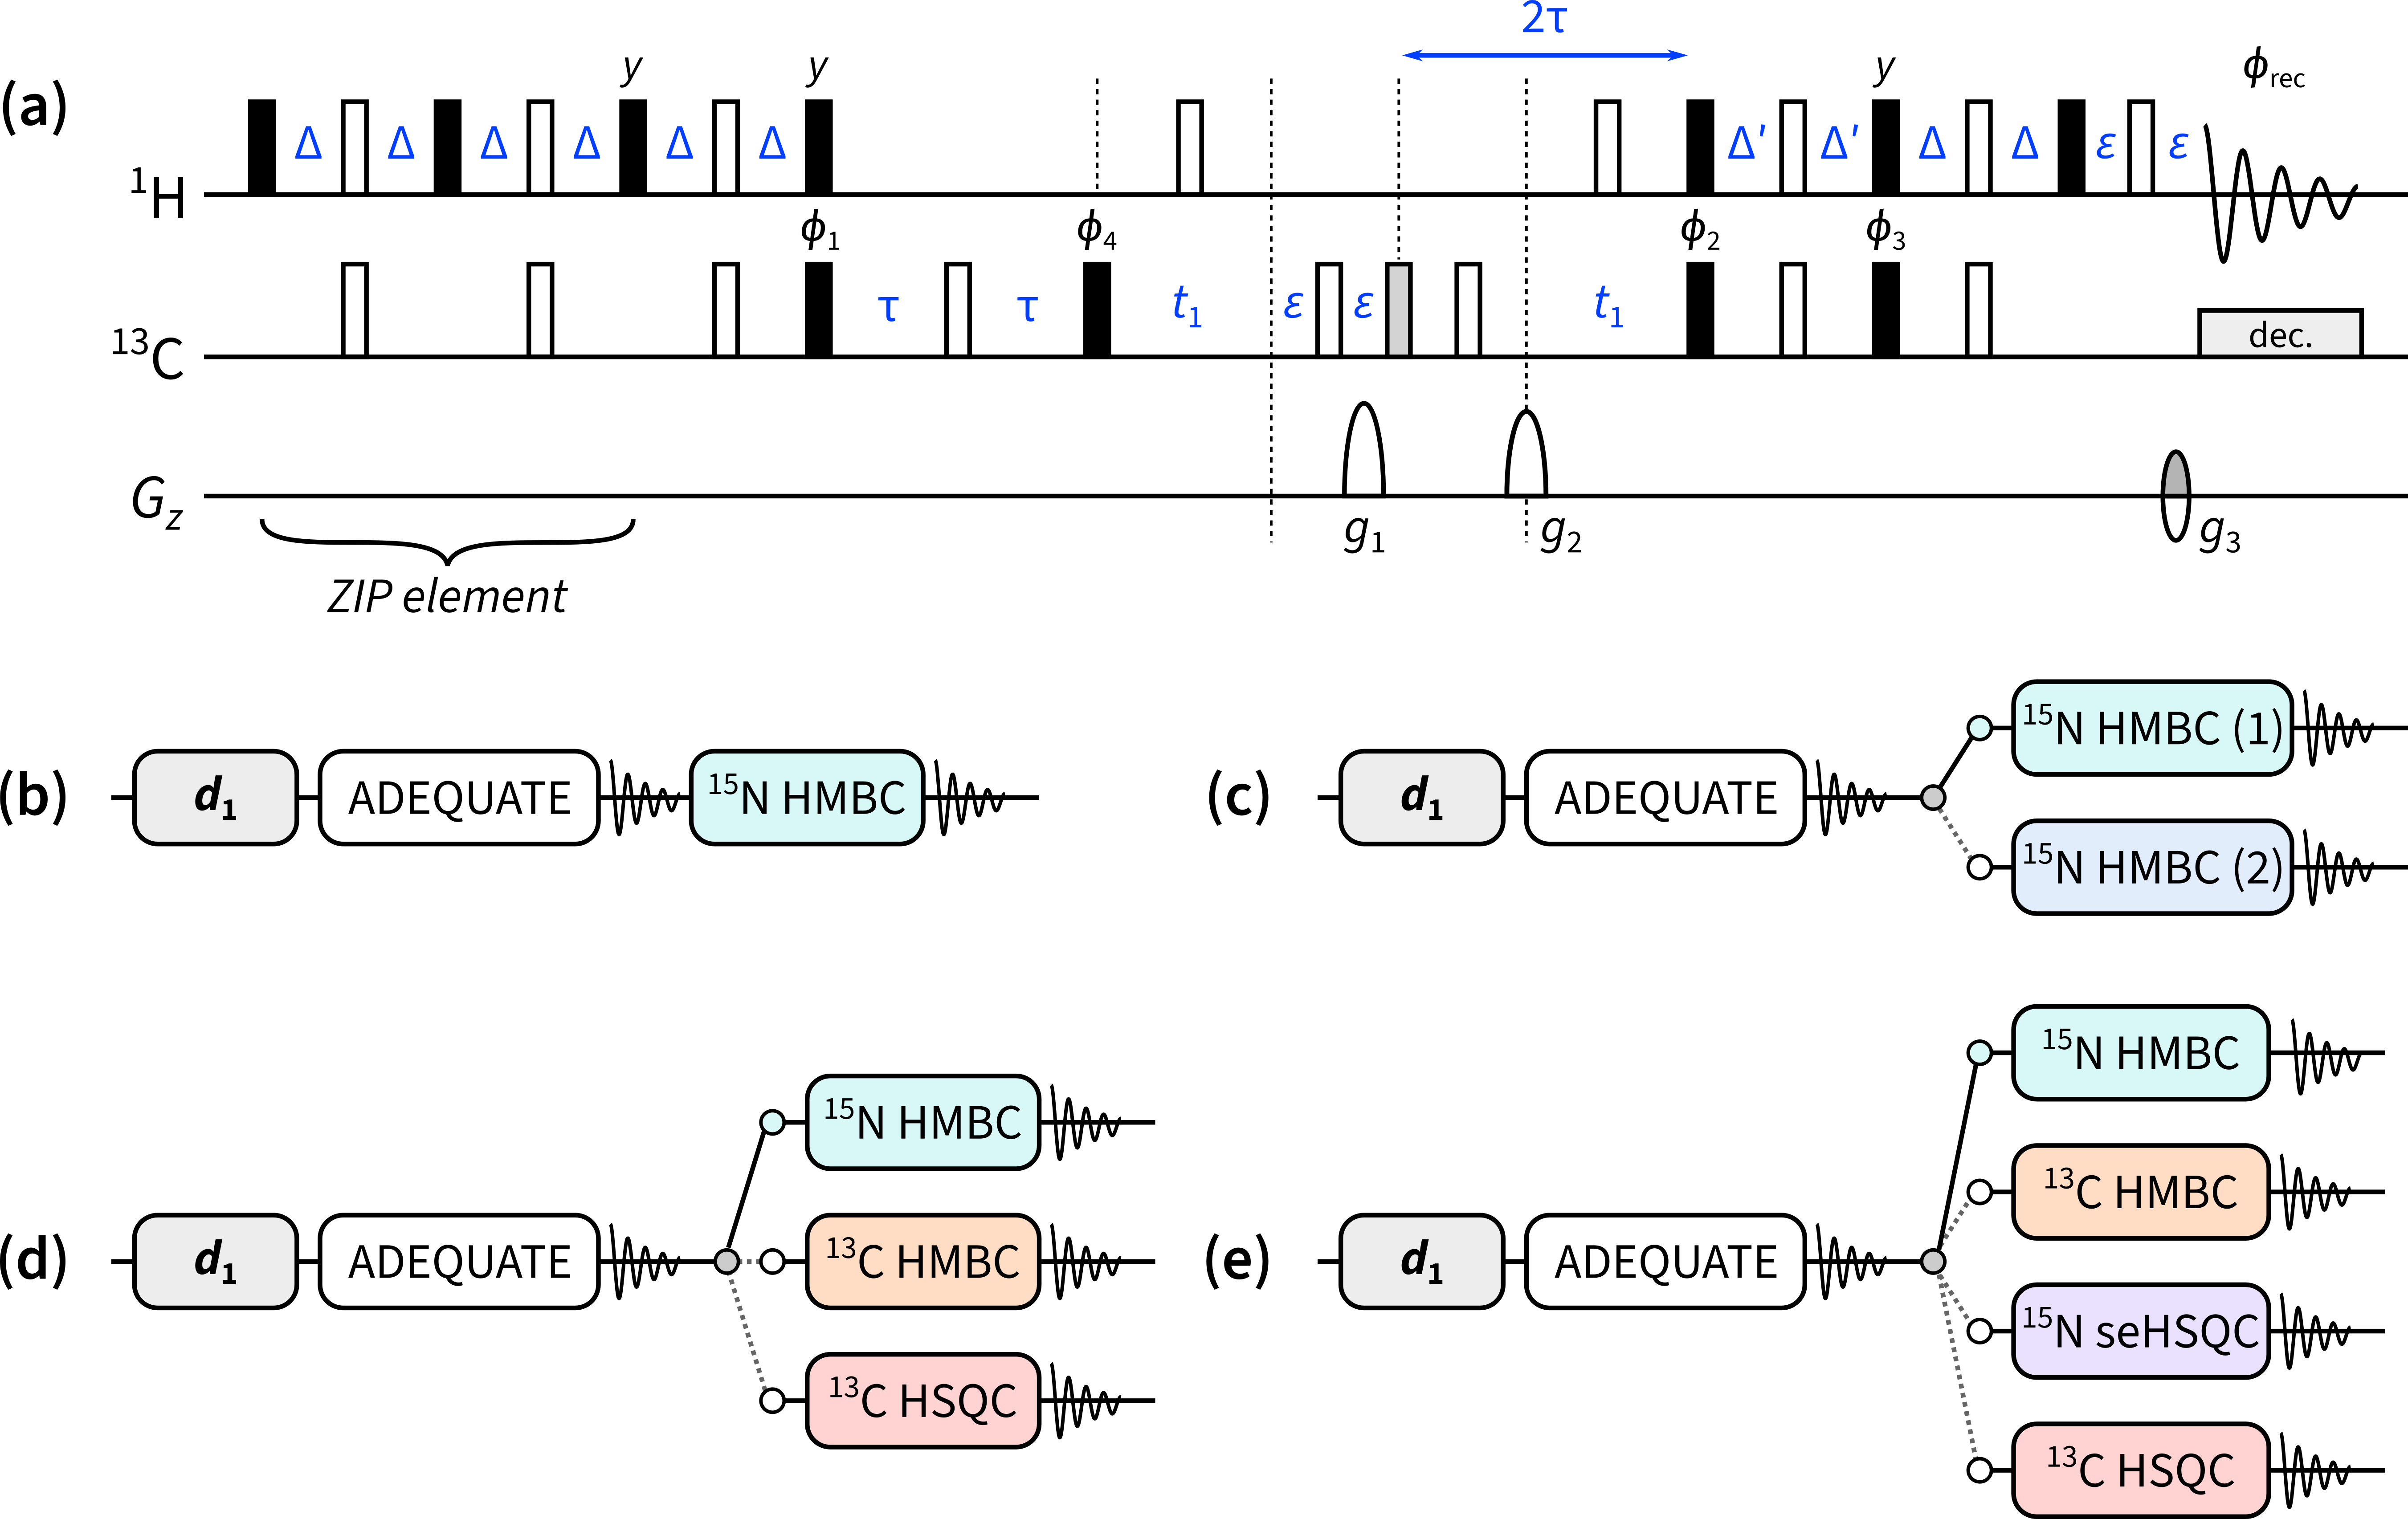
\includegraphics[width=\textwidth]{sequences.png}
    {\phantomsubcaption\label{fig:sequences_adequate}}
    {\phantomsubcaption\label{fig:sequences_ab}}
    {\phantomsubcaption\label{fig:sequences_abb}}
    {\phantomsubcaption\label{fig:sequences_abbs}}
    {\phantomsubcaption\label{fig:sequences_abbss}}
    \caption{
        Pulse sequences described in this work.
        \textbf{(\subref{fig:sequences_adequate})} ZIP-1,1-ADEQUATE module.
        Filled and empty bars refer to \ang{90} and \ang{180} pulses respectively; the grey filled bar is a \ang{120} pulse for \carbon{} double-quantum to single-quantum coherence transfer\autocite{Mareci1982JMR}.
        Pulse and receiver phases are: $\phi_1 = x, -x$; $\phi_2 = 2\,(x), 2\,(-x)$; $\phi_3 = 2\,(y), 2\,(-y)$; $\phi_4 = 4\,(x), 4\,(-x)$; $\phi_\text{rec} = x, -x, -x, x, -x, x, x, -x$.
        Delays are set as follows: $\Delta = 1 / (4 \cdot \onejch)$, $\Delta' = 1 / (8 \cdot \onejch)$, and $\tau = 1 / (4 \cdot \onejcc)$. $\varepsilon$ is the minimum time required for a pulsed field gradient and the following recovery delay.
        Gradient amplitudes as a percentage of the maximum amplitude (\SI{53}{G/cm}) are: $g_1 = 78.5\%$, $g_2 = 77.6\%$, and $g_3 = -59\%$.
        Echo--antiecho selection is achieved by inverting the sign of $g_3$ as well as the pulse phase $\phi_3$.
        \textbf{(\subref{fig:sequences_ab})} NOAH-2 \noahtwo{A}{Bn} supersequence.
        \textbf{(\subref{fig:sequences_abb})} NOAH-3 \noahthree{A}{Bn}{Bn}, where the two \nitrogen{} HMBC experiments are optimised for two different values of $\njnh{}$.
        \textbf{(\subref{fig:sequences_abbs})} NOAH-4 \noahfour{A}{Bn}{B}{S}.
        \textbf{(\subref{fig:sequences_abbss})} NOAH-5 \noahfive{A}{Bn}{B}{Spn}{S}.
    }
    \label{fig:sequences}
\end{figure}

\section{NOAH-2 AB\texorpdfstring{$_{\ch{N}}$}{n}}

When designing NMR supersequences, it is generally a good rule of thumb to place the module with the lowest sensitivity first: this is because any incomplete preservation of magnetisation by earlier modules will lead to decreased sensitivity in later modules.
The 1,1-ADEQUATE module, which relies on neighbouring pairs of \carbon{} isotopes---occurring only in roughly 1 out of 8130 molecules---therefore forms the beginning of all the supersequences described here.

The ADEQUATE module (\cref{fig:sequences_adequate}) is designed to only use the magnetisation of protons directly bonded to \carbon{}, which we denote here as \magn{\ch{C}}.\autocite{Orts2018M,Yong2021JMR}
In order to maintain the sensitivity of later modules, it must return the magnetisation of all other protons (denoted as \magnnot{\ch{C}}) to the equilibrium $+z$ state.
This is accomplished by replacing the initial \ang{90} excitation pulse by the $zz$-isotope selective pulse element (ZIP)\autocite{Hansen2021AC,Yong2021JMR}, which effects $90^\circ_{-x}$ and $90^\circ_{-y}$ rotations on \magn{\ch{C}} and \magnnot{\ch{C}} magnetisation respectively.
(Other isotope-specific elements such as BANGO\autocite{Sorensen1994BMR,Nagy2019CC,Nagy2021ACIE} may also be used here, with similar results generally being obtained.\autocite{Yong2021JMR})
The \nitrogen{} HMBC module of choice is a simple magnitude-mode version, with an optional first-order low-pass J-filter.
In the NOAH-2 \noahtwo{A}{Bn} supersequence (ADEQUATE + \nitrogen{} HMBC, \cref{fig:sequences_ab}), this module simply consumes the remaining \magnnot{\ch{C}} magnetisation which was preserved by the ZIP-ADEQUATE.

\begin{figure}[ht]
    \centering
    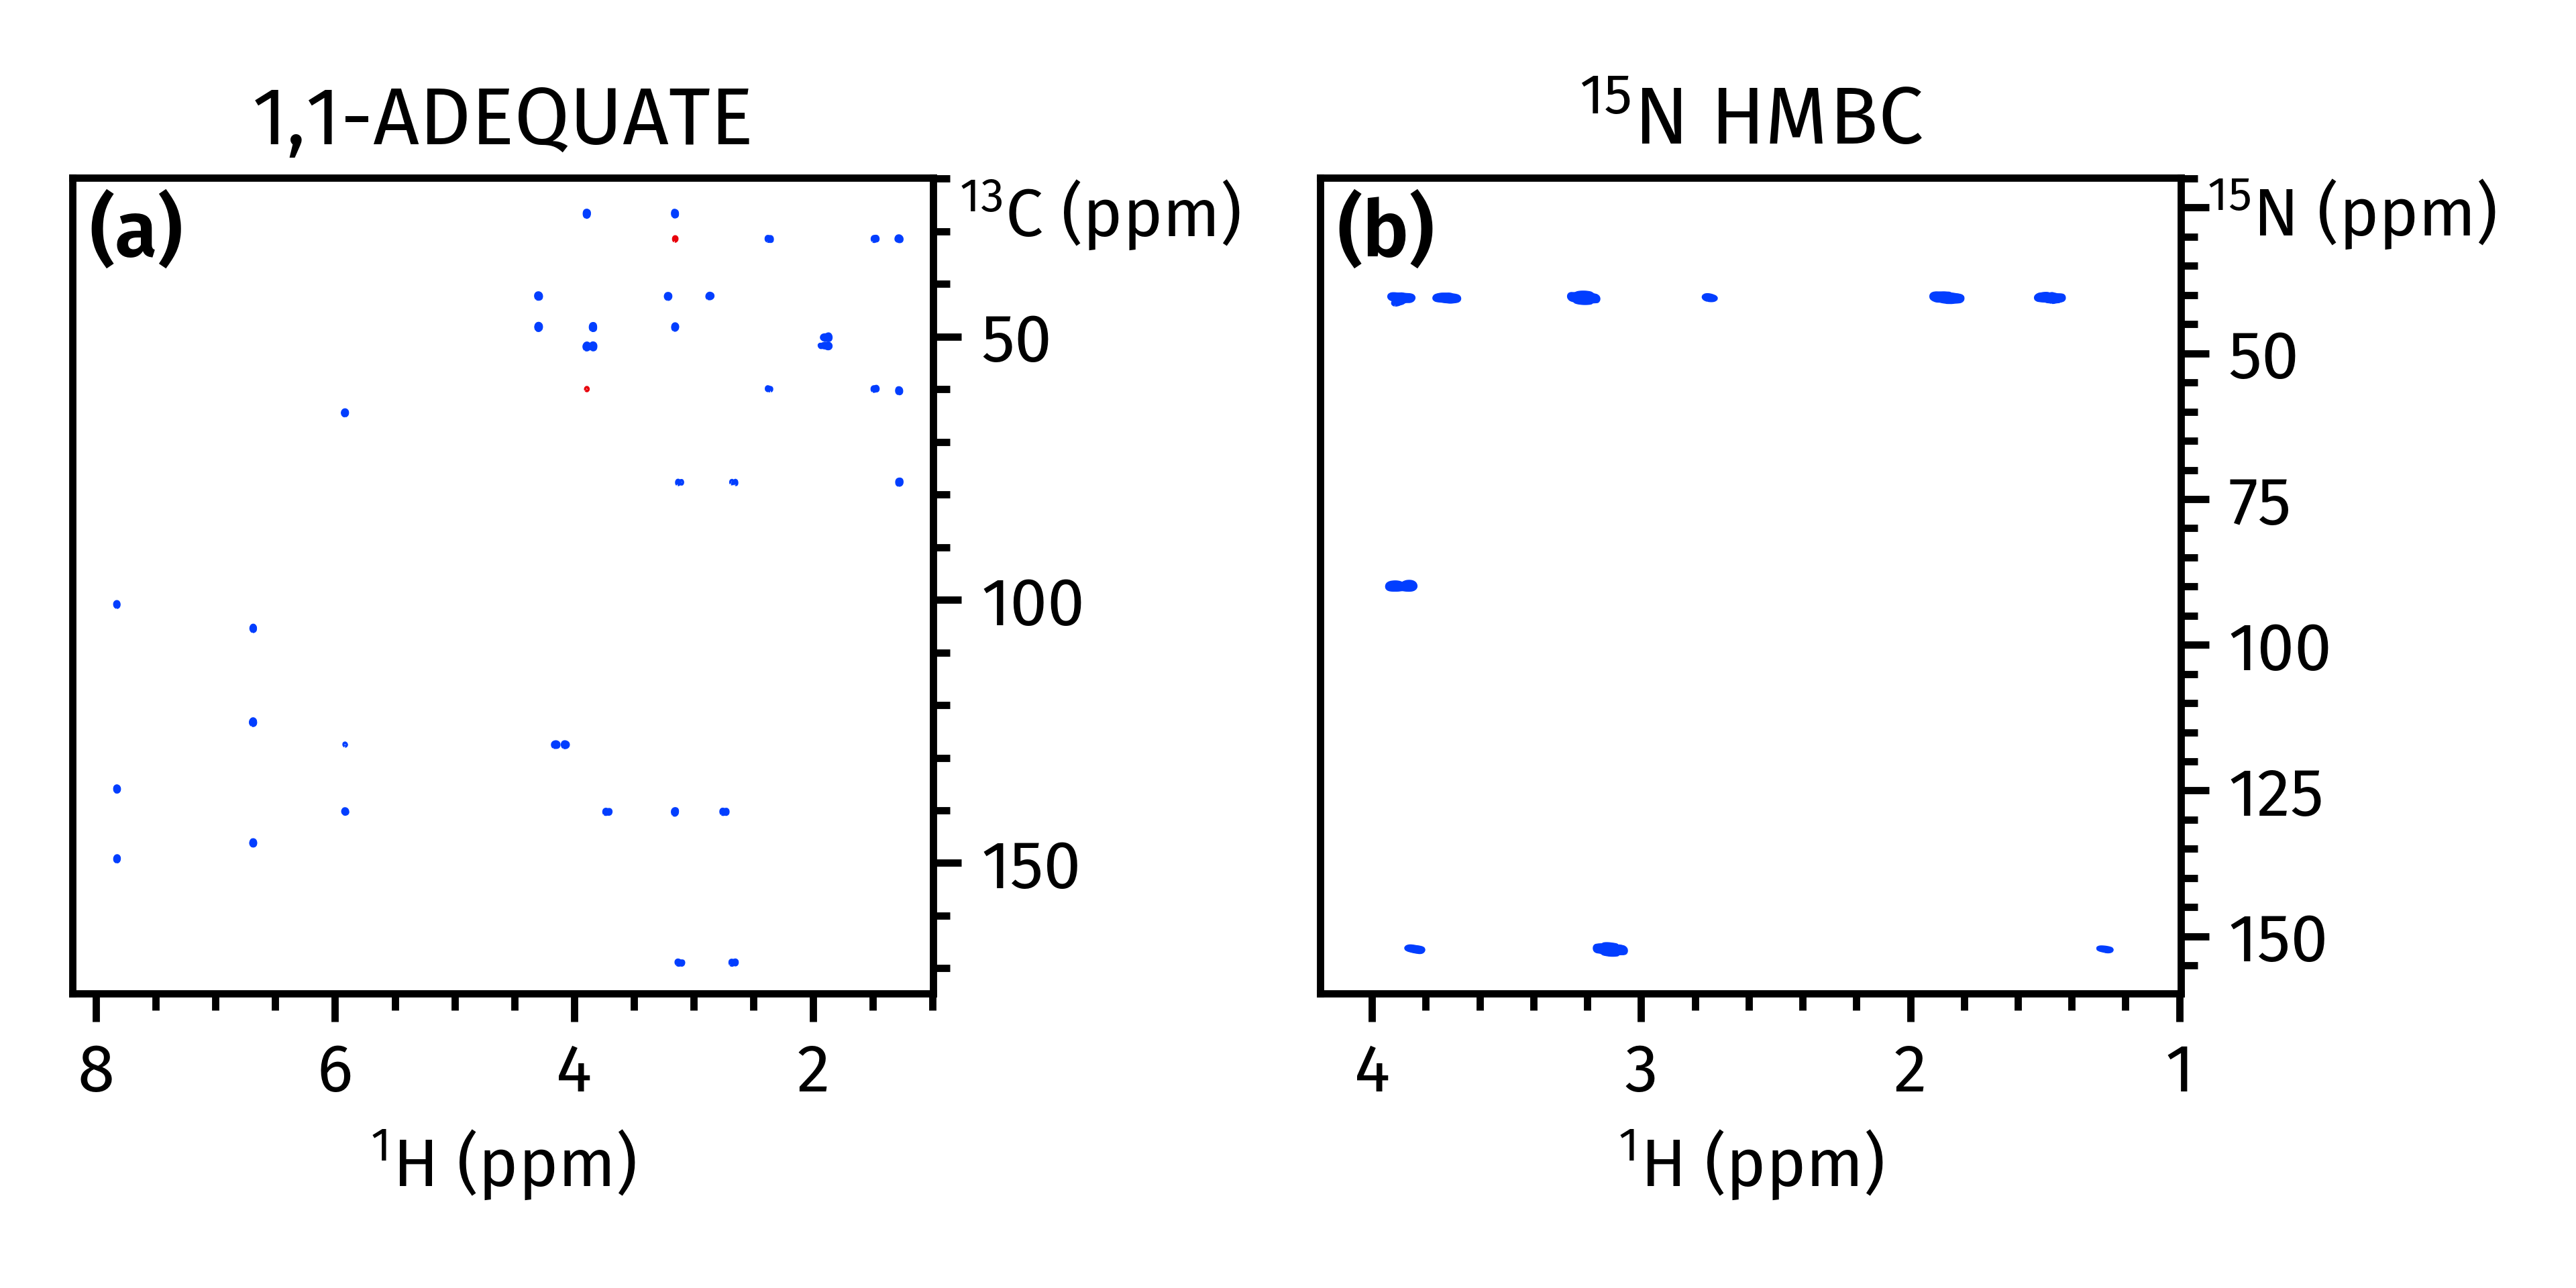
\includegraphics[width=0.7\textwidth]{ab.png}
    {\phantomsubcaption\label{fig:ab_adeq}}
    {\phantomsubcaption\label{fig:ab_n_hmbc}}
    \caption{
        Spectra obtained from the NOAH-2 \noahtwo{A}{Bn} supersequence.
        \textbf{(\subref{fig:ab_adeq})} 1,1-ADEQUATE.
        \textbf{(\subref{fig:ab_n_hmbc})} \nitrogen{} HMBC.
        \brucine{}
    }
    \label{fig:ab}
\end{figure}


\section{NOAH-3 AB\texorpdfstring{$_{\ch{N}}$}{n}B\texorpdfstring{$_{\ch{N}}$}{n}}

Although this sequence on its own performs well (\cref{fig:ab}), it suffers from the drawback that the \nitrogen{} HMBC is optimised for one specific value of $\njnh$.
In practice, $\njnh{}$ values range from \qtyrange{2}{16}{Hz}; in a single HMBC experiment, some correlations may therefore be lost due to J-coupling mismatch.

To circumvent this issue, a variety of accordion-type experiments\autociteset{accordion_hmbc} have been designed which decrement the J-evolution period in step with $t_1$, allowing a wider range of couplings to be sampled.
Here, we adopt the simpler approach of recording two separate HMBC experiments optimised for different $\njnh$ values.
This cannot be performed \textit{sequentially} as the two HMBC experiments would draw on the same \magnnot{\ch{C}} magnetisation, causing the second to suffer from severely decreased sensitivity.
However, they can easily be done in an \textit{interleaved} manner where, after the ADEQUATE module, the two HMBC experiments are alternately acquired (\cref{fig:sequences_abb}).\autocite{Kupce2021JACSA}
As the \nitrogen{} dimension is typically sparse and a high resolution is not required, we choose to run both \nitrogen{} HMBC spectra with half the usual number of $t_1$ increments compared to the ADEQUATE.
As can be seen in \cref{fig:abb}, the two HMBC spectra reveal different sets of correlations.

\begin{figure}[ht]
    \centering
    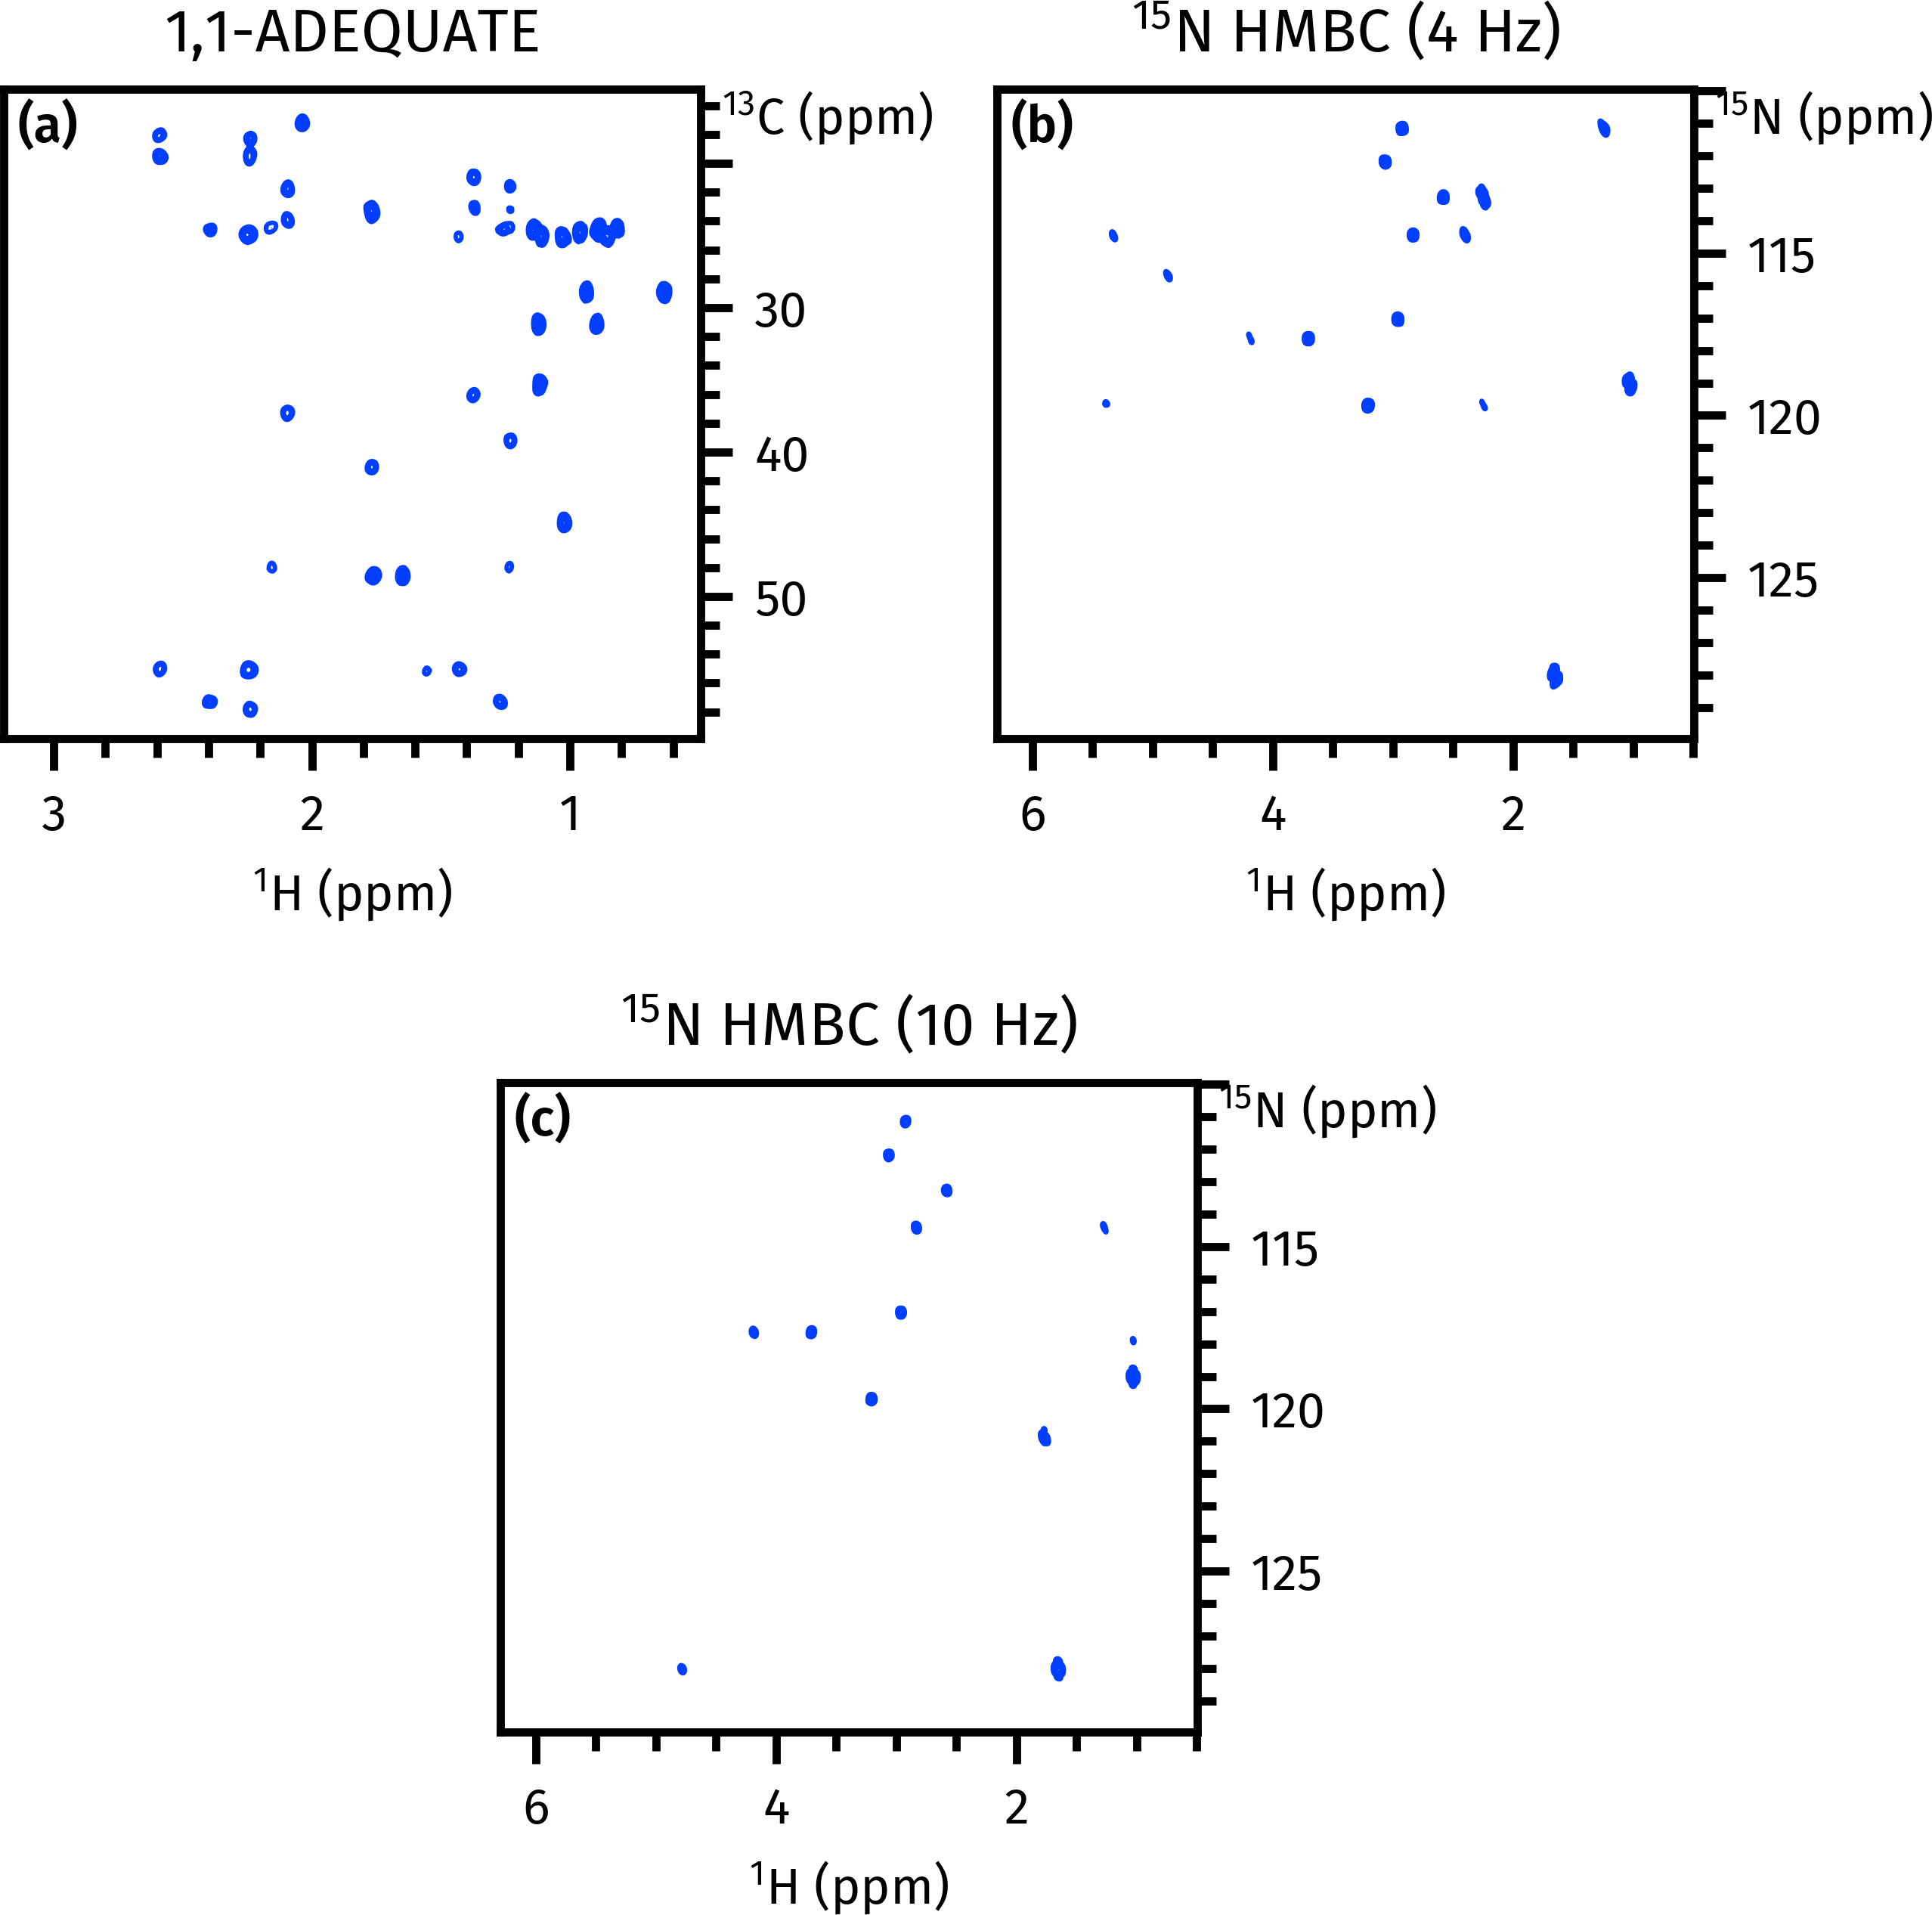
\includegraphics[width=\textwidth]{abb.png}
    {\phantomsubcaption\label{fig:abb_adeq}}
    {\phantomsubcaption\label{fig:abb_n_hmbc1}}
    {\phantomsubcaption\label{fig:abb_n_hmbc2}}
    \caption{
        Spectra obtained from the NOAH-3 \noahthree{A}{Bn}{Bn} supersequence.
        \textbf{(\subref{fig:abb_adeq})} 1,1-ADEQUATE (256 $t_1$ increments).
        \textbf{(\subref{fig:abb_n_hmbc1})} \nitrogen{} HMBC optimised for $\njnh = \SI{4}{Hz}$ (128 $t_1$ increments).
        \textbf{(\subref{fig:abb_n_hmbc2})} \nitrogen{} HMBC optimised for $\njnh = \SI{10}{Hz}$ (128 $t_1$ increments).
        \cyclo{}
    }
    \label{fig:abb}
\end{figure}

\section{NOAH-4 AB\texorpdfstring{$_{\ch{N}}$}{n}BS}

In the above spectra and in previous work,\autocite{Kupce2021JACSA} we have shown how two alternating modules can be used to construct parallel supersequences.
Naturally, this concept can be further generalised to use $N \geq 2$ alternating `threads'.
This is demonstrated using the NOAH-4 \noahfour{A}{Bn}{B}{S} supersequence (\cref{fig:sequences_abbs}), in which the ADEQUATE module is followed by either a \nitrogen{} HMBC, \carbon{} HMBC, or \carbon{} HSQC.
Because these three latter modules do not have the same intrinsic sensitivity, we balance this by allocating a different number of threads to each module.
For example, with $N = 8$, we can acquire the \nitrogen{} HMBC six times and the \carbon{} HMBC and HSQC once each.
After summation of the data, this effectively amounts to acquiring the ADEQUATE experiment with $8n$ transients, the \nitrogen{} HMBC with $6n$ transients, and the \carbon{} HMBC and HSQC with $n$ transients each (where $n$ is some positive integer).
This particular ratio yielded the spectra shown in \cref{fig:abbs}; the user may also customise these numbers themselves using the pulse programmes provided in the \SInf{}.

\begin{figure}[ht]
    \centering
    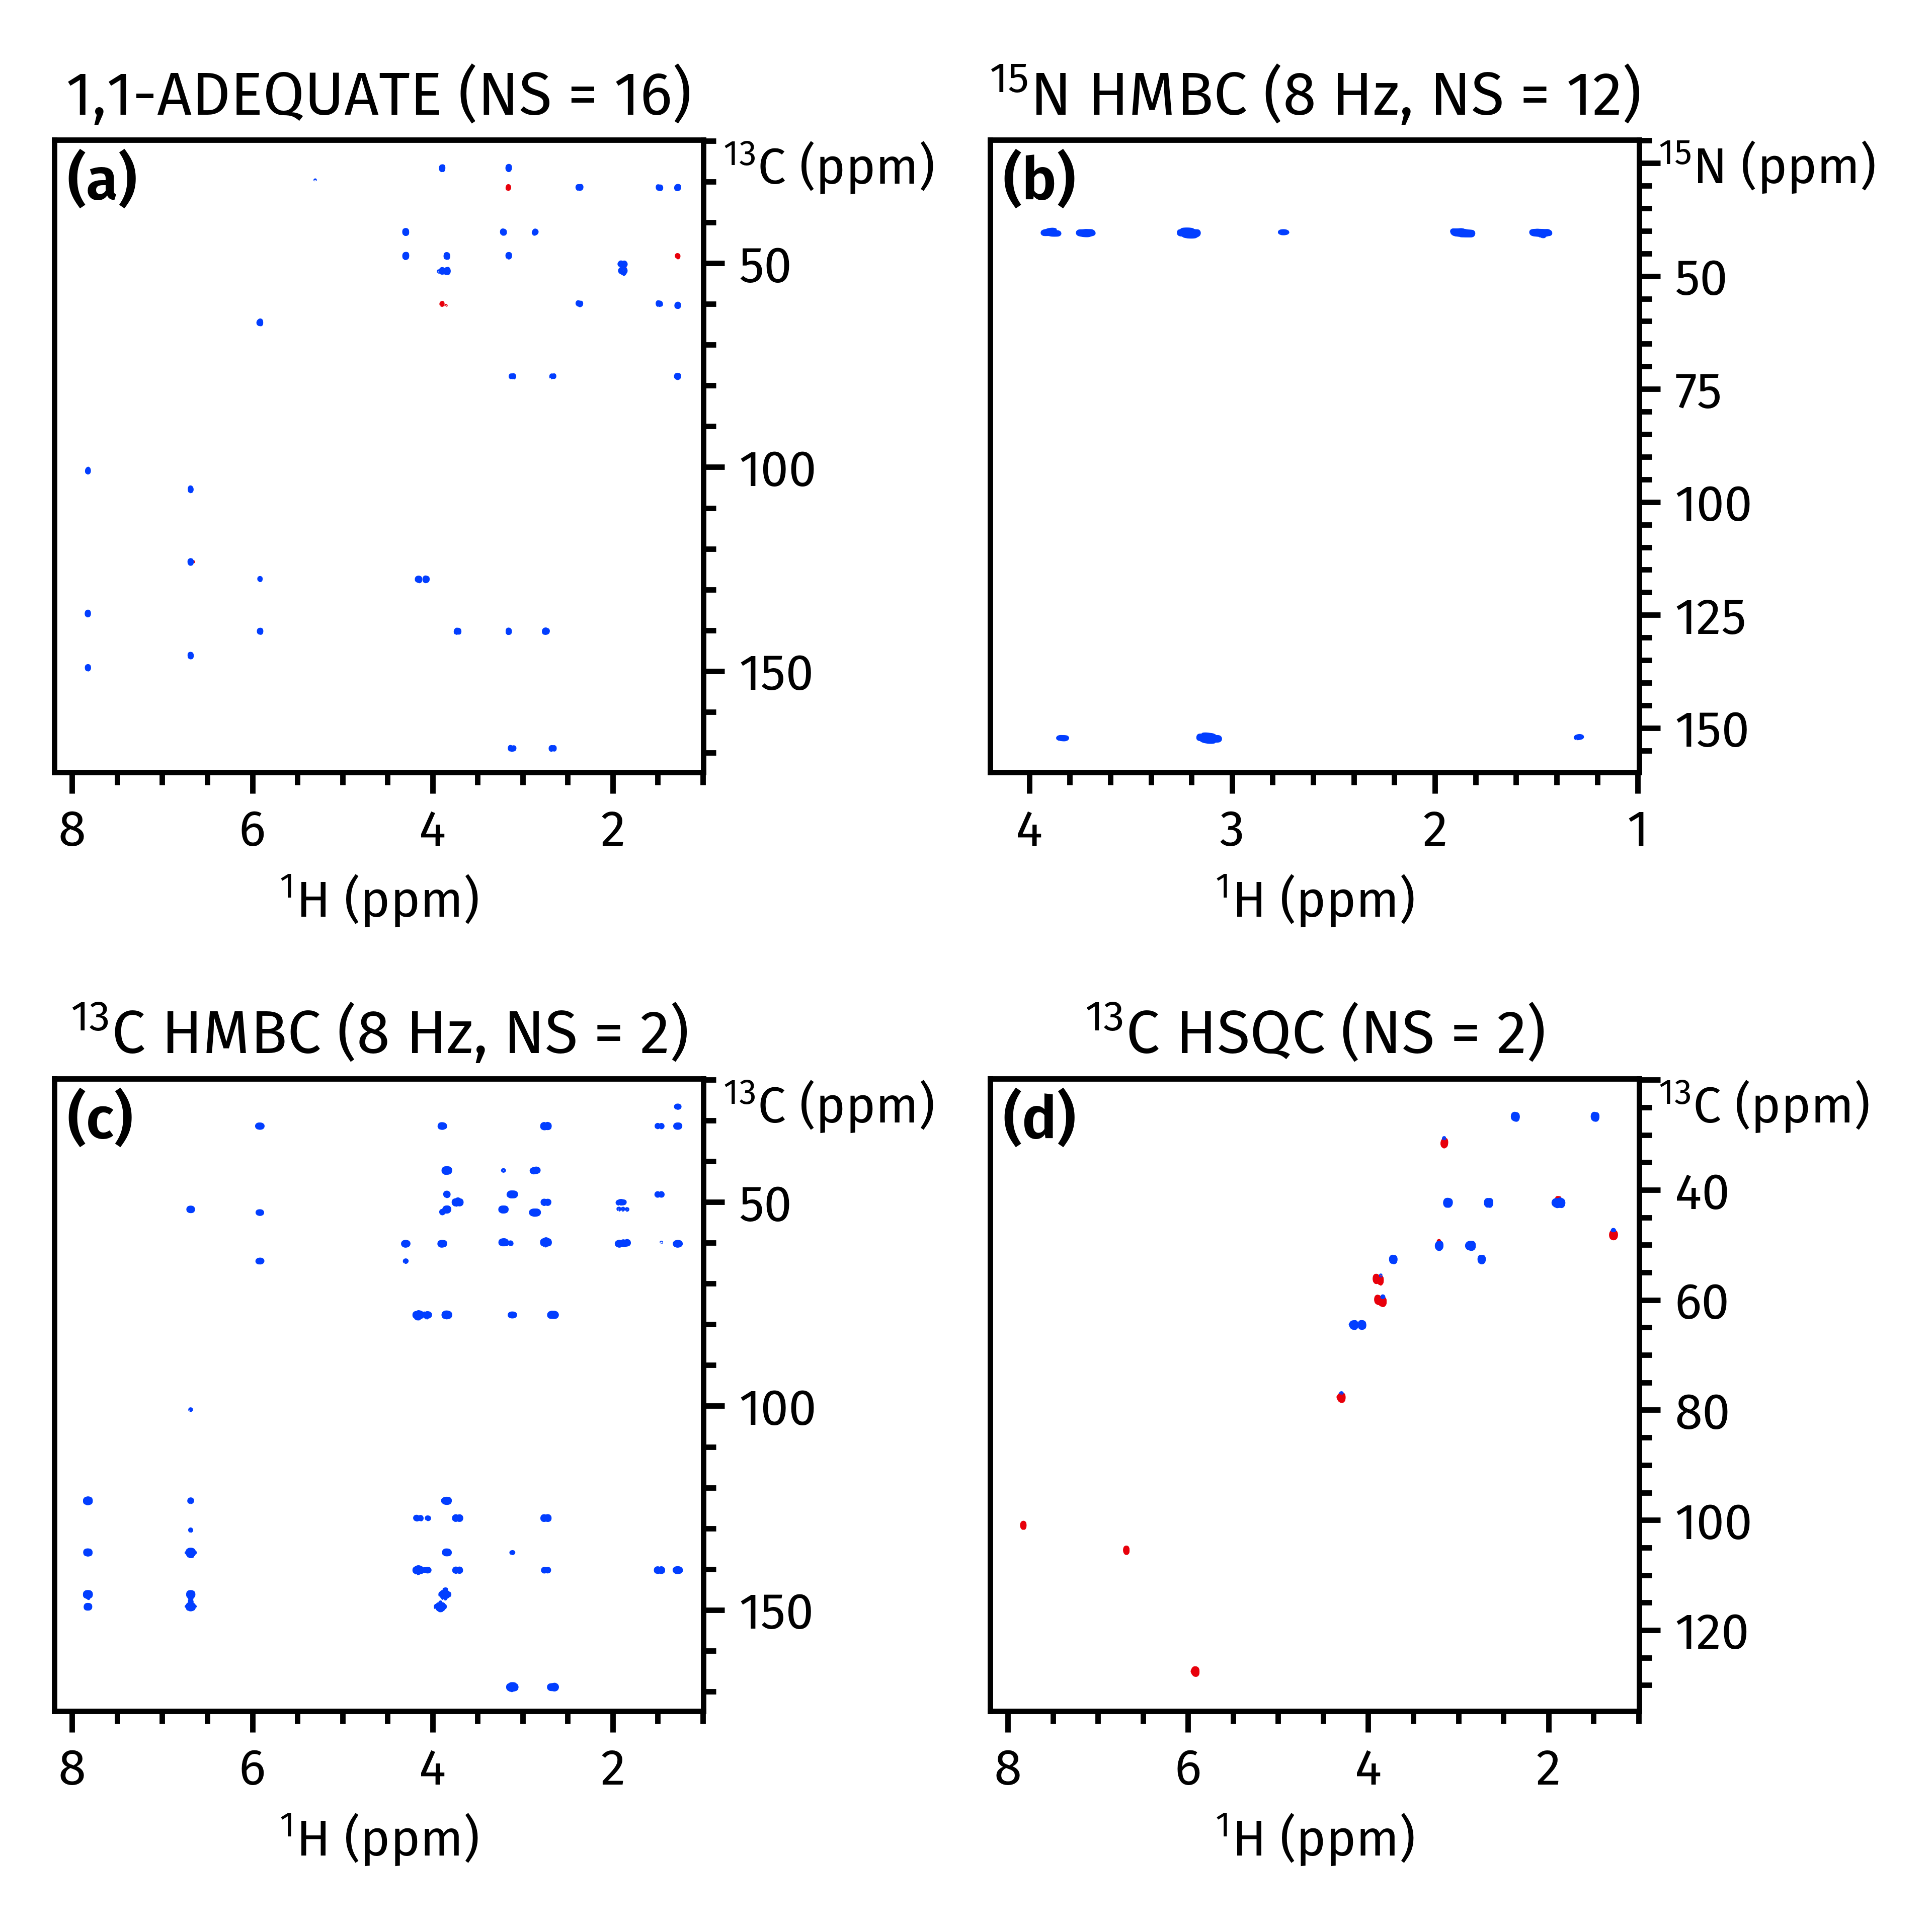
\includegraphics[width=0.7\textwidth]{abbs.png}
    {\phantomsubcaption\label{fig:abbs_adeq}}
    {\phantomsubcaption\label{fig:abbs_n_hmbc}}
    {\phantomsubcaption\label{fig:abbs_c_hmbc}}
    {\phantomsubcaption\label{fig:abbs_c_hsqc}}
    \caption{
        Spectra obtained from the NOAH-4 \noahfour{A}{Bn}{B}{S} supersequence.
        \textbf{(\subref{fig:abbs_adeq})} 1,1-ADEQUATE (16 transients).
        \textbf{(\subref{fig:abbs_n_hmbc})} \nitrogen{} HMBC (12 transients).
        \textbf{(\subref{fig:abbs_c_hmbc})} \carbon{} HMBC (2 transients).
        \textbf{(\subref{fig:abbs_c_hsqc})} \carbon{} HSQC (2 transients).
        \brucine{}
    }
    \label{fig:abbs}
\end{figure}

Like the \nitrogen{} HMBC, the \carbon{} HMBC module simply use up all the \magnnot{\ch{C}} magnetisation preserved by the ADEQUATE.
However, the \carbon{} HSQC draws on the same \magn{\ch{C}} magnetisation pool.
In order to increase the sensitivity of the HSQC experiment, we add a period of isotropic DIPSI-2 mixing\autocite{Shaka1988JMR} immediately before the HSQC module to effect \magnnot{\ch{C}} $\to$ \magn{\ch{C}} magnetisation transfer, as has previously been done in ASAP\autociteset{asaphsqc} and NOAH\autocite{Yong2021JMR} experiments (\cref{fig:dipsi}).

The acquisition of the NOAH-4 \noahfour{A}{Bn}{B}{S} spectra in \cref{fig:abbs} took 124 minutes; in contrast, normal acquisition of all four experiments (with the appropriate number of transients) required a total of 223 minutes.
As the ADEQUATE is placed first in the supersequence, its sensitivity is almost identical to that of a standalone ADEQUATE; the inclusion of the ZIP element does not have an appreciable impact on this. \todo{\textit{[Not sure why; we clearly saw at least 10\% loss in seHSQC.]}}
The two HMBC spectra experience small losses \todo{(16--36\%)} in sensitivity, due to imperfect magnetisation retention by the ADEQUATE module.
This is, however, outweighed by the almost twofold time savings provided by concatenation of the modules: if the NOAH supersequence were acquired for as long as the standalone experiments would, the \nitrogen{} and \carbon{} HMBC spectra would in fact have \todo{$-14$\%} and \todo{12\%} increases in SNR respectively.
\todo{\textit{
[The numbers are placeholders for now, reason being that the ABBS expt was acquired with 2.5 ms gradients in \nitrogen{} HMBC---this leads to a 36\% loss compared to the standalone \nitrogen{} HMBC which was acquired with 1 ms gradients.
The \carbon{} HMBC loses 16\% which is about right.
I don't think the longer gradients are} really \textit{necessary, so I'd prefer to redo the experiment to get nicer numbers.]
}}
Due to the reuse of \magn{\ch{C}} magnetisation, the HSQC module only retains 32\% of its original sensitivity.
However, as the HSQC is still two orders of magnitude more sensitive than the ADEQUATE, this decrease is readily tolerated; if necessary, the sensitivity-enhanced HSQC module\autocite{Palmer1991JMR,Kay1992JACS,Hansen2021AC,Yong2021JMR} may also be used in its place.

\section{NOAH-5 AB\texorpdfstring{$_{\ch{N}}$}{n}BS\texorpdfstring{$^+_{\ch{N}}$}{+n}S}

As a final example, we add a further \nitrogen{} seHSQC module to the above sequence.
This is most easily accomplished by simply diverting one `thread' away from the \nitrogen{} HMBC, meaning that the second slot in the supersequence now alternates between four different experiment (\cref{fig:sequences_abbss}).
In principle, the \nitrogen{} seHSQC uses only \magn{\ch{N}} magnetisation (i.e.\ protons directly bonded to \nitrogen{}), and can simply be added as a third module in every `thread` of the supersequence: such an arrangement would maximise its sensitivity as a larger number of transients are collected.
However, this would compromise the performance of the \textit{other} modules, as they must then be modified to preserve this magnetisation: for example, the HMBC modules would need to include the $zz$-filter\autocite{Kupce2018CC,Kupce2019JMR}, which generally causes 10--20\% sensitivity losses.
As the \nitrogen{} seHSQC is not a particularly demanding experiment in terms of sensitivity, it makes more sense to implement it in this interleaved manner.
This example especially illustrates how the use of interleaved \textit{and} sequential acquisition leads to much greater flexibility in supersequence design, especially when considering the relative sensitivities of different modules.

\begin{figure}[ht]
    \centering
    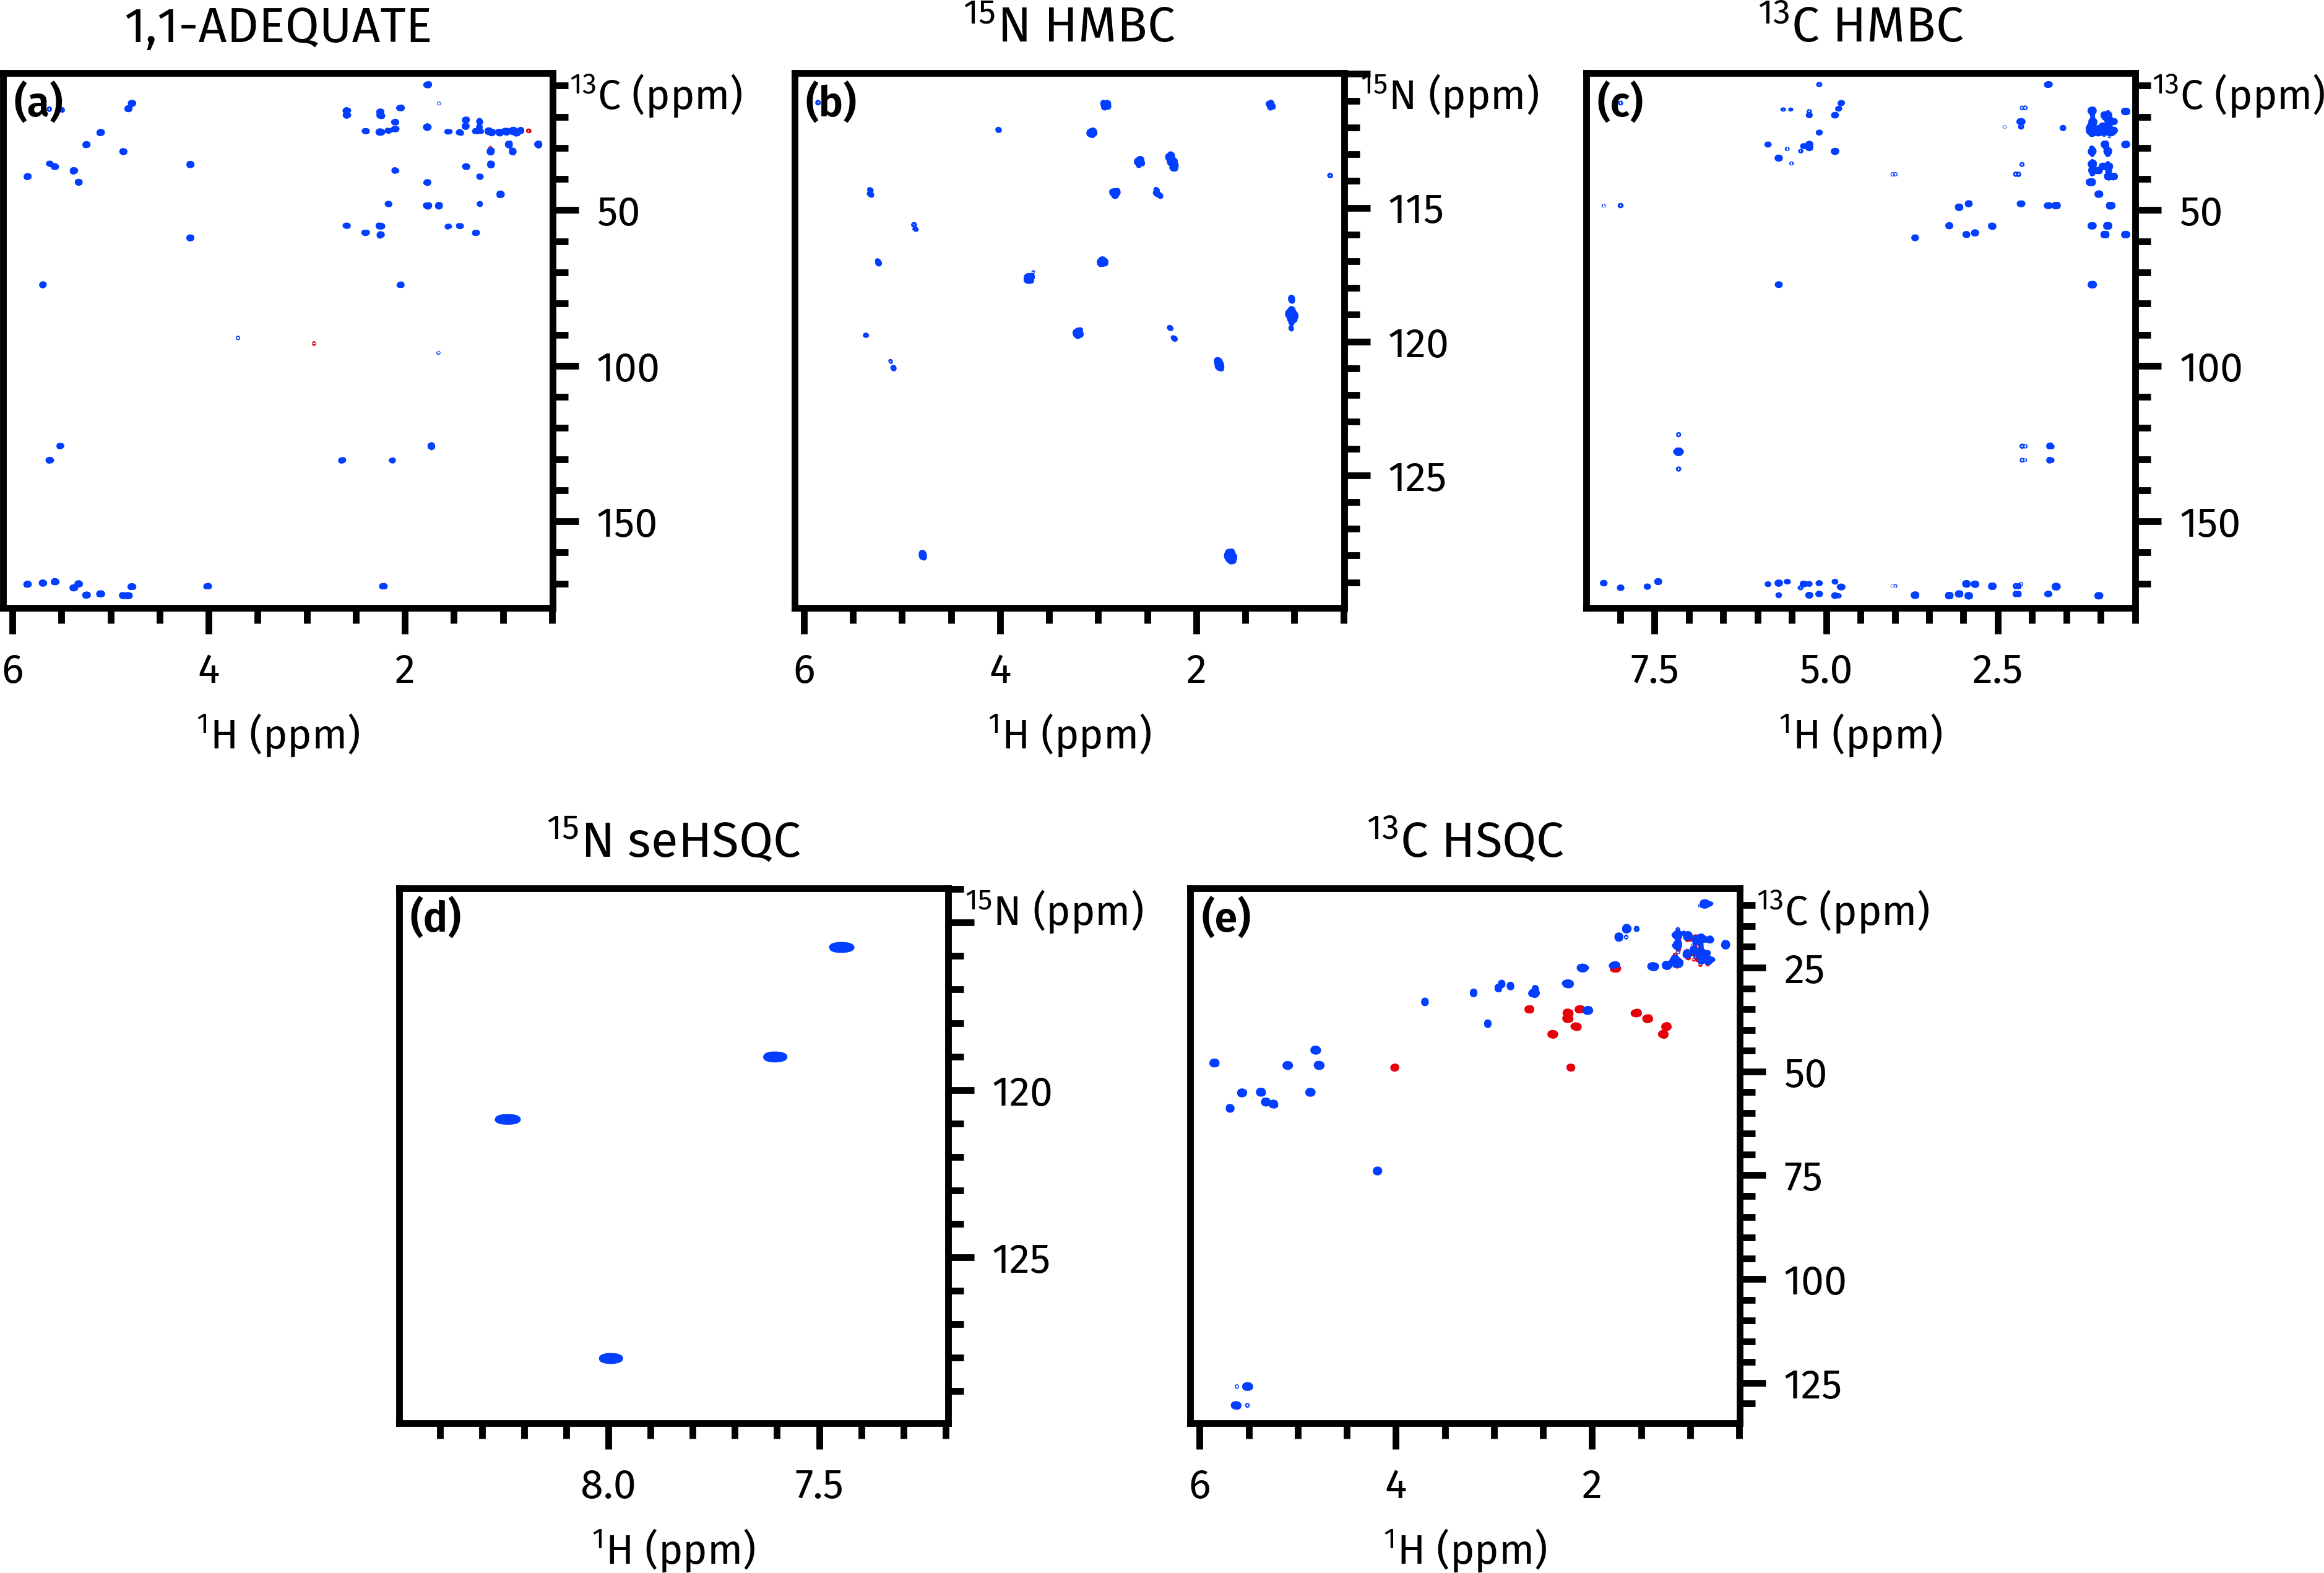
\includegraphics[width=\textwidth]{abbss.png}
    {\phantomsubcaption\label{fig:abbss_adeq}}
    {\phantomsubcaption\label{fig:abbss_n_hmbc}}
    {\phantomsubcaption\label{fig:abbss_c_hmbc}}
    {\phantomsubcaption\label{fig:abbss_n_sehsqc}}
    {\phantomsubcaption\label{fig:abbss_c_hsqc}}
    \caption{
        Spectra obtained from the NOAH-5 \noahfive{A}{Bn}{B}{Spn}{S} supersequence.
        \textbf{(\subref{fig:abbss_adeq})} 1,1-ADEQUATE (16 transients).
        \textbf{(\subref{fig:abbss_n_hmbc})} \nitrogen{} HMBC (10 transients).
        \textbf{(\subref{fig:abbss_c_hmbc})} \carbon{} HMBC (2 transients).
        \textbf{(\subref{fig:abbss_n_sehsqc})} \nitrogen{} sensitivity-enhanced HSQC (2 transients).
        \textbf{(\subref{fig:abbss_c_hsqc})} \carbon{} HSQC (2 transients).
        \cyclo{}
    }
    \label{fig:abbss}
\end{figure}

The five spectra thus obtained are shown in \cref{fig:abbss}.
Collectively, this supersequence provides virtually all heteronuclear correlation data required for structural elucidation or assignment.
This is similar in spirit to the PANACEA experiment\autociteset{panacea}, but yields greater sensitivity as it uses equilibrium \proton{} magnetisation rather than the low-magnetogyric ratio \carbon{} and \nitrogen{} nuclei, and does not require multiple-receiver hardware.\autocite{Kupce2021PNMRS,Kupce2021NRMP}

\begin{figure}[ht]
    \centering
    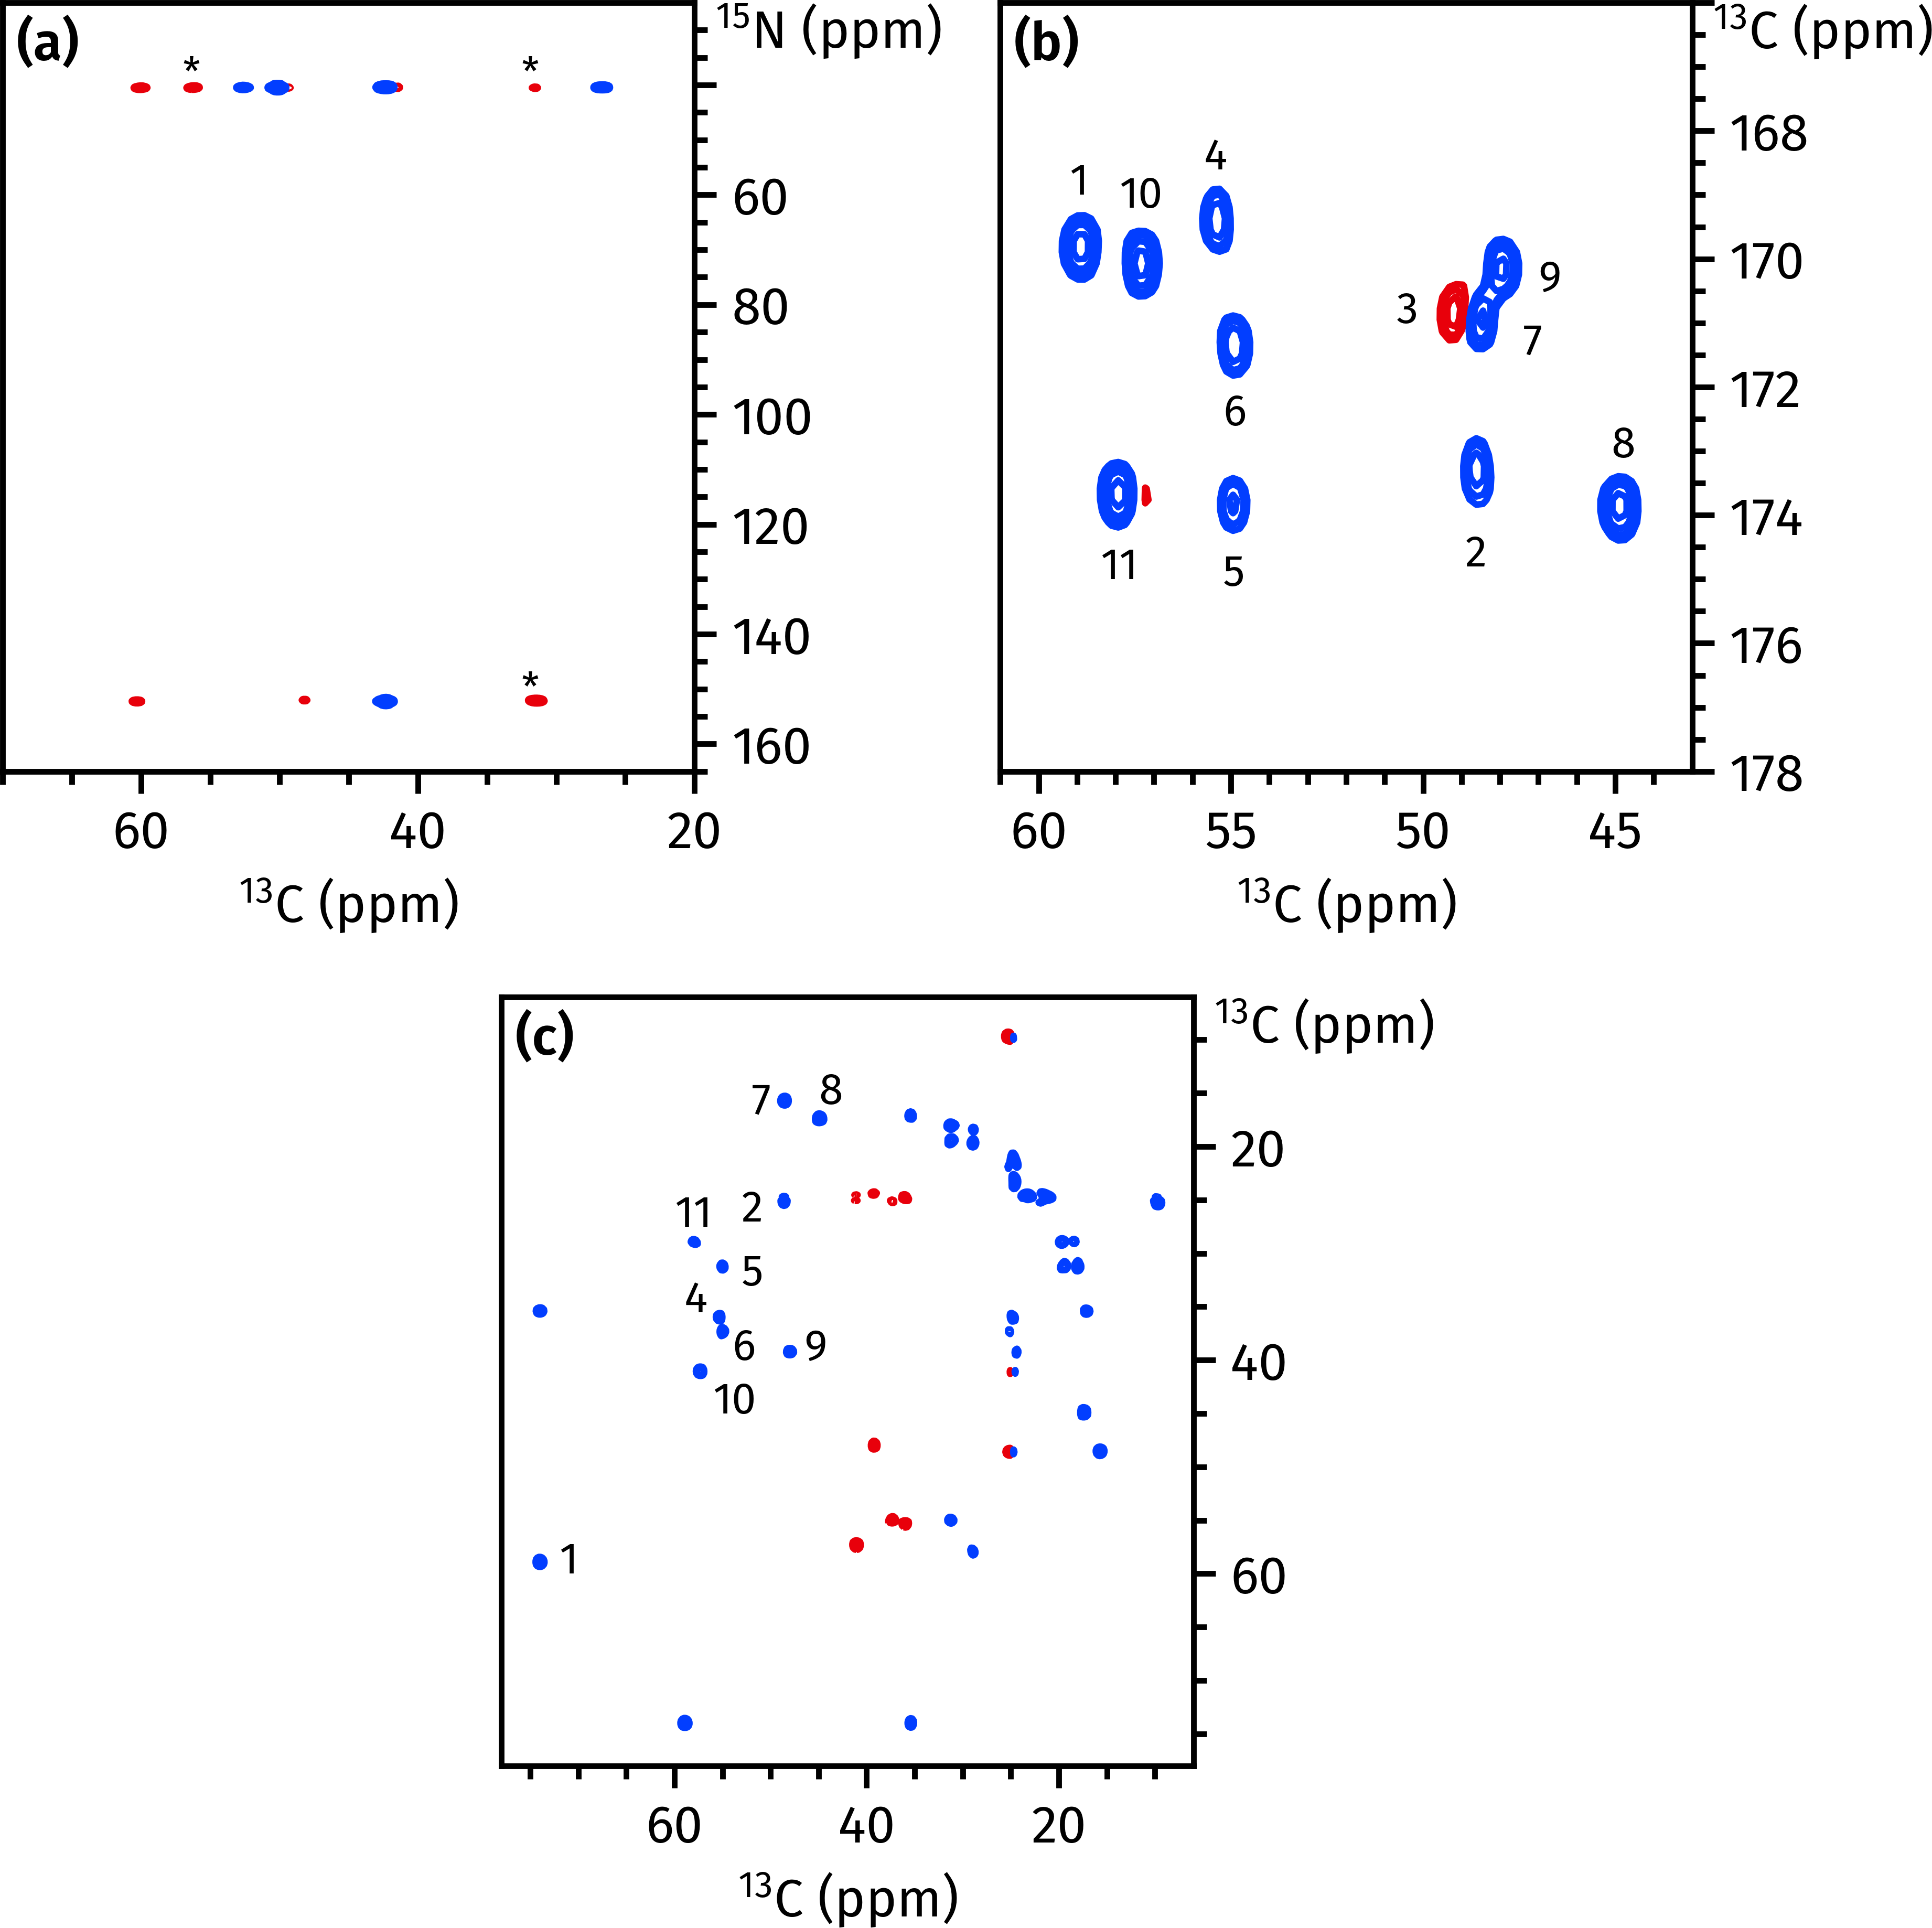
\includegraphics[width=\textwidth]{covariance.png}
    {\phantomsubcaption\label{fig:covariance_brucine_nc}}
    {\phantomsubcaption\label{fig:covariance_cyclo_caco}}
    {\phantomsubcaption\label{fig:covariance_cyclo_sidechain}}
    \caption{
        Spectra obtained through indirect covariance processing.
        \textbf{(\subref{fig:covariance_brucine_nc})} \carbon{}--\nitrogen{} correlation spectrum (containing both one- and multiple-bond correlations) obtained by processing the brucine \nitrogen{} HMBC and \carbon{} HSQC spectra (in \cref{fig:abbs_n_hmbc,fig:abbs_c_hsqc}) using unsymmetric indirect covariance.
        \textbf{(\subref{fig:covariance_cyclo_caco}--\subref{fig:covariance_cyclo_sidechain})} Insets of \carbon{}--\carbon{} one-bond correlation spectrum, obtained by processing the cyclosporin ADEQUATE and \carbon{} HSQC spectra (in \cref{fig:abbss_adeq,fig:abbss_c_hsqc}) using generalised indirect covariance ($\lambda = 0.5$).
        The \ch{C}$\alpha$--\ch{CO} correlations are shown in (\subref{fig:covariance_cyclo_caco}), and sidechain \ch{C-C} correlations in (\subref{fig:covariance_cyclo_sidechain}).
        \todo{(\textit{Some} of the peaks in (a) and (c) are artefacts. (b) is very satisfying though---11 peaks for 11 residues. I assigned every peak except for those in the top-right corner of (c)... we \textit{could} crop (c) to show only C$\alpha$--C$\beta$ correlations, which I did completely assign.)}
    }
    \label{fig:covariance}
\end{figure}

It is possible to further combine these spectra using indirect covariance processing\autociteset{indirect-covariance} to generate other forms of correlation spectra.
For example, when processed in this way, the \nitrogen{} HMBC and \carbon{} HSQC yield \carbon{}--\nitrogen{} correlation spectra.\autociteset{cn-covariance}
Furthermore, the \carbon{} HSQC and ADEQUATE experiments can be used to create \carbon{}--\carbon{} one-bond correlation spectra.\autociteset{hsqc-adequate}
It should be further emphasised that all of the `base' spectra used as the inputs here are obtained \textit{in a single measurement} using either the NOAH-4 or NOAH-5 supersequences discussed above.

\section{Conclusion(ish)}

While the generalised supersequences presented here enable modules to be assembled in almost any imaginable way, their increasing complexity mean that pulse programme construction is more difficult.
At present, the GENESIS tool for automatic pulse sequence generation\autocite{Yong2022AC} only provides limited options for parallel supersequences.
In particular, it is restricted to only \textit{two} different `threads' (as demonstrated in previous work\autocite{Kupce2021JACSA}); we hope to expand this in the near future.
Different AU programmes are also required to process the data correctly.
The pulse sequences and processing scripts used in this work are provided in the Bruker User Library, accessible at \url{https://www.bruker.com/en/services/bruker-user-library.html}.

In conclusion, we have demonstrated here how low-sensitivity experiments, such as 1,1-ADEQUATE and \nitrogen{} HMBC, may be combined in NMR supersequences, leading to substantial reductions in experiment time.
Using the principles of sequential and interleaved acquisition, further high-sensitivity modules may be added almost at will through a generalisation of our previous concept of `parallel' supersequences, where multiple `threads' are executed and divided between several interleaved modules.
The spectra thus obtained provide the chemist with far more powerful tools for the characterisation of complex molecules, especially in cases where existing NOAH supersequences do not provide sufficient information for unambiguous assignment.

\section*{Acknowledgements}

We thank Dr Mohammadali Foroozandeh (University of Oxford) for helpful discussions.
J.R.J.Y.\ thanks the Clarendon Fund (University of Oxford) and the EPSRC Centre for Doctoral Training in Synthesis for Biology and Medicine (EP/L015838/1) for a studentship, generously supported by AstraZeneca, Diamond Light Source, Defence Science and Technology Laboratory, Evotec, GlaxoSmithKline, Janssen, Novartis, Pfizer, Syngenta, Takeda, UCB, and Vertex.

% Fakesection Bibliography
\AtNextBibliography{\small}
\printbibliography{}
\end{refsection}


% Fakesection ================= SI ==================

\clearpage
\begin{refsection}
\newcommand{\sectionbreak}{\clearpage}
\renewcommand*{\thefigure}{S\arabic{figure}}
\renewcommand*{\thesection}{S\arabic{section}}
\renewcommand*{\thetable}{S\arabic{table}}
\renewcommand*{\thepage}{S\arabic{page}}
\setcounter{page}{1}
\setcounter{figure}{0}
\setcounter{section}{0}
\setcounter{table}{0}
\onehalfspacing

\hspace{0pt}
\vfill
\begin{center}
    \huge
    Supporting Information

    \vspace{0.3cm}

    \textit{for}

    \vspace{0.3cm}

    \articletitle{}

    \vspace{0.6cm}

    \Large Jonathan R.\ J.\ Yong,\textsuperscript{1} {\=E}riks Kup{\v{c}}e,\textsuperscript{2} Tim D.\ W.\ Claridge\textsuperscript{1,\texttt{*}}

    \vspace{0.6cm}

    \large \textsuperscript{1} \textit{\crl{}}

    \textsuperscript{2} \textit{\brukeruk{}}

    \textsuperscript{\texttt{*}} \texttt{tim.claridge@chem.ox.ac.uk}

\end{center}

\vspace{2cm}
\section*{Contents}

\startcontents[si]
\printcontents[si]{ }{1}{}
\vfill
\hspace{0pt}
\newpage

\section{Pulse programme description}

With a more detailed diagram \& explanation

\section{Pulse programme setup}

For ABBS, the thought process is generally as follows:

\begin{itemize}
    \item Decide on number of $t_1$ increments for each module (we call this $N_1$). This is determined by desired resolution in indirect dimension. Say 256.
    \item Decide on NS for each module. NS for ADEQUATE must be equal to sum of NS for all other modules.
    \item Determine the gcd of the separate NS's (for example, gcd(16, 12, 2, 2) = 2). Set the TopSpin parameter \texttt{NS} as this value. Make sure this is at least 2 as this determines the minimum phase cycle
    \item Set (\texttt{cnst51}, \texttt{cnst52}, \texttt{cnst53}, \texttt{cnst54}) = NS's divided through by their gcd (so 8, 6, 1, 1). In practice the last of these is automatically calculated, so it doesn't have to be set.
    \item Set \texttt{NBL} = 2 since there are only really two `horizontally' combined modules.
    \item Set TopSpin \texttt{TD1} parameter to be $N_1$ $\times$ \texttt{NBL} $\times$ \texttt{cnst51}. In this case, $256 \times 2 \times 8 = 4096$.
\end{itemize}

\todo{
    Should note here that previous parallel supersequences\autocite{Kupce2021JACSA} essentially follow the same idea but with two threads.
    The sequences don't explicitly use the \texttt{cnst} parameters as shown above, but in practice they behave exactly as if \texttt{cnst51} = 2 and \texttt{cnst52} = \texttt{cnst53} = 1.

    This observation, in principle, should open up a `path' to generalising the GENESIS algorithm---but I need time to do it.
    Providing a GUI is also problematic.
    (I have some \textit{ideas} about the desired UI, but actually \textit{implementing} it is another matter\ldots{})
}



\section{Spectra that didn't make it into the main text}

\todo{(We should move some figures from the main text to here---the only question is which ones?}

Since the \proton{}--\proton{} NOESY uses the same \magnnot{\ch{C}} magnetisation as \carbon{} HMBC so can be directly substituted in its place, leading to a NOAH-4 \noahfour{A}{Bn}{N}{S} supersequence (\cref{fig:abns}).
This not only provides a wealth of through-bond correlations which aid in eludicating molecular constitution, but also furnishes through-space correlations for the determination of configuration or conformation.

\todo{One \textit{actual} problem here is the receiver gain. For ABBS I had $\texttt{RG} = 2050$, but for this I had to set $\texttt{RG} = 29$(!!).}

\begin{figure}[ht]
    \centering
    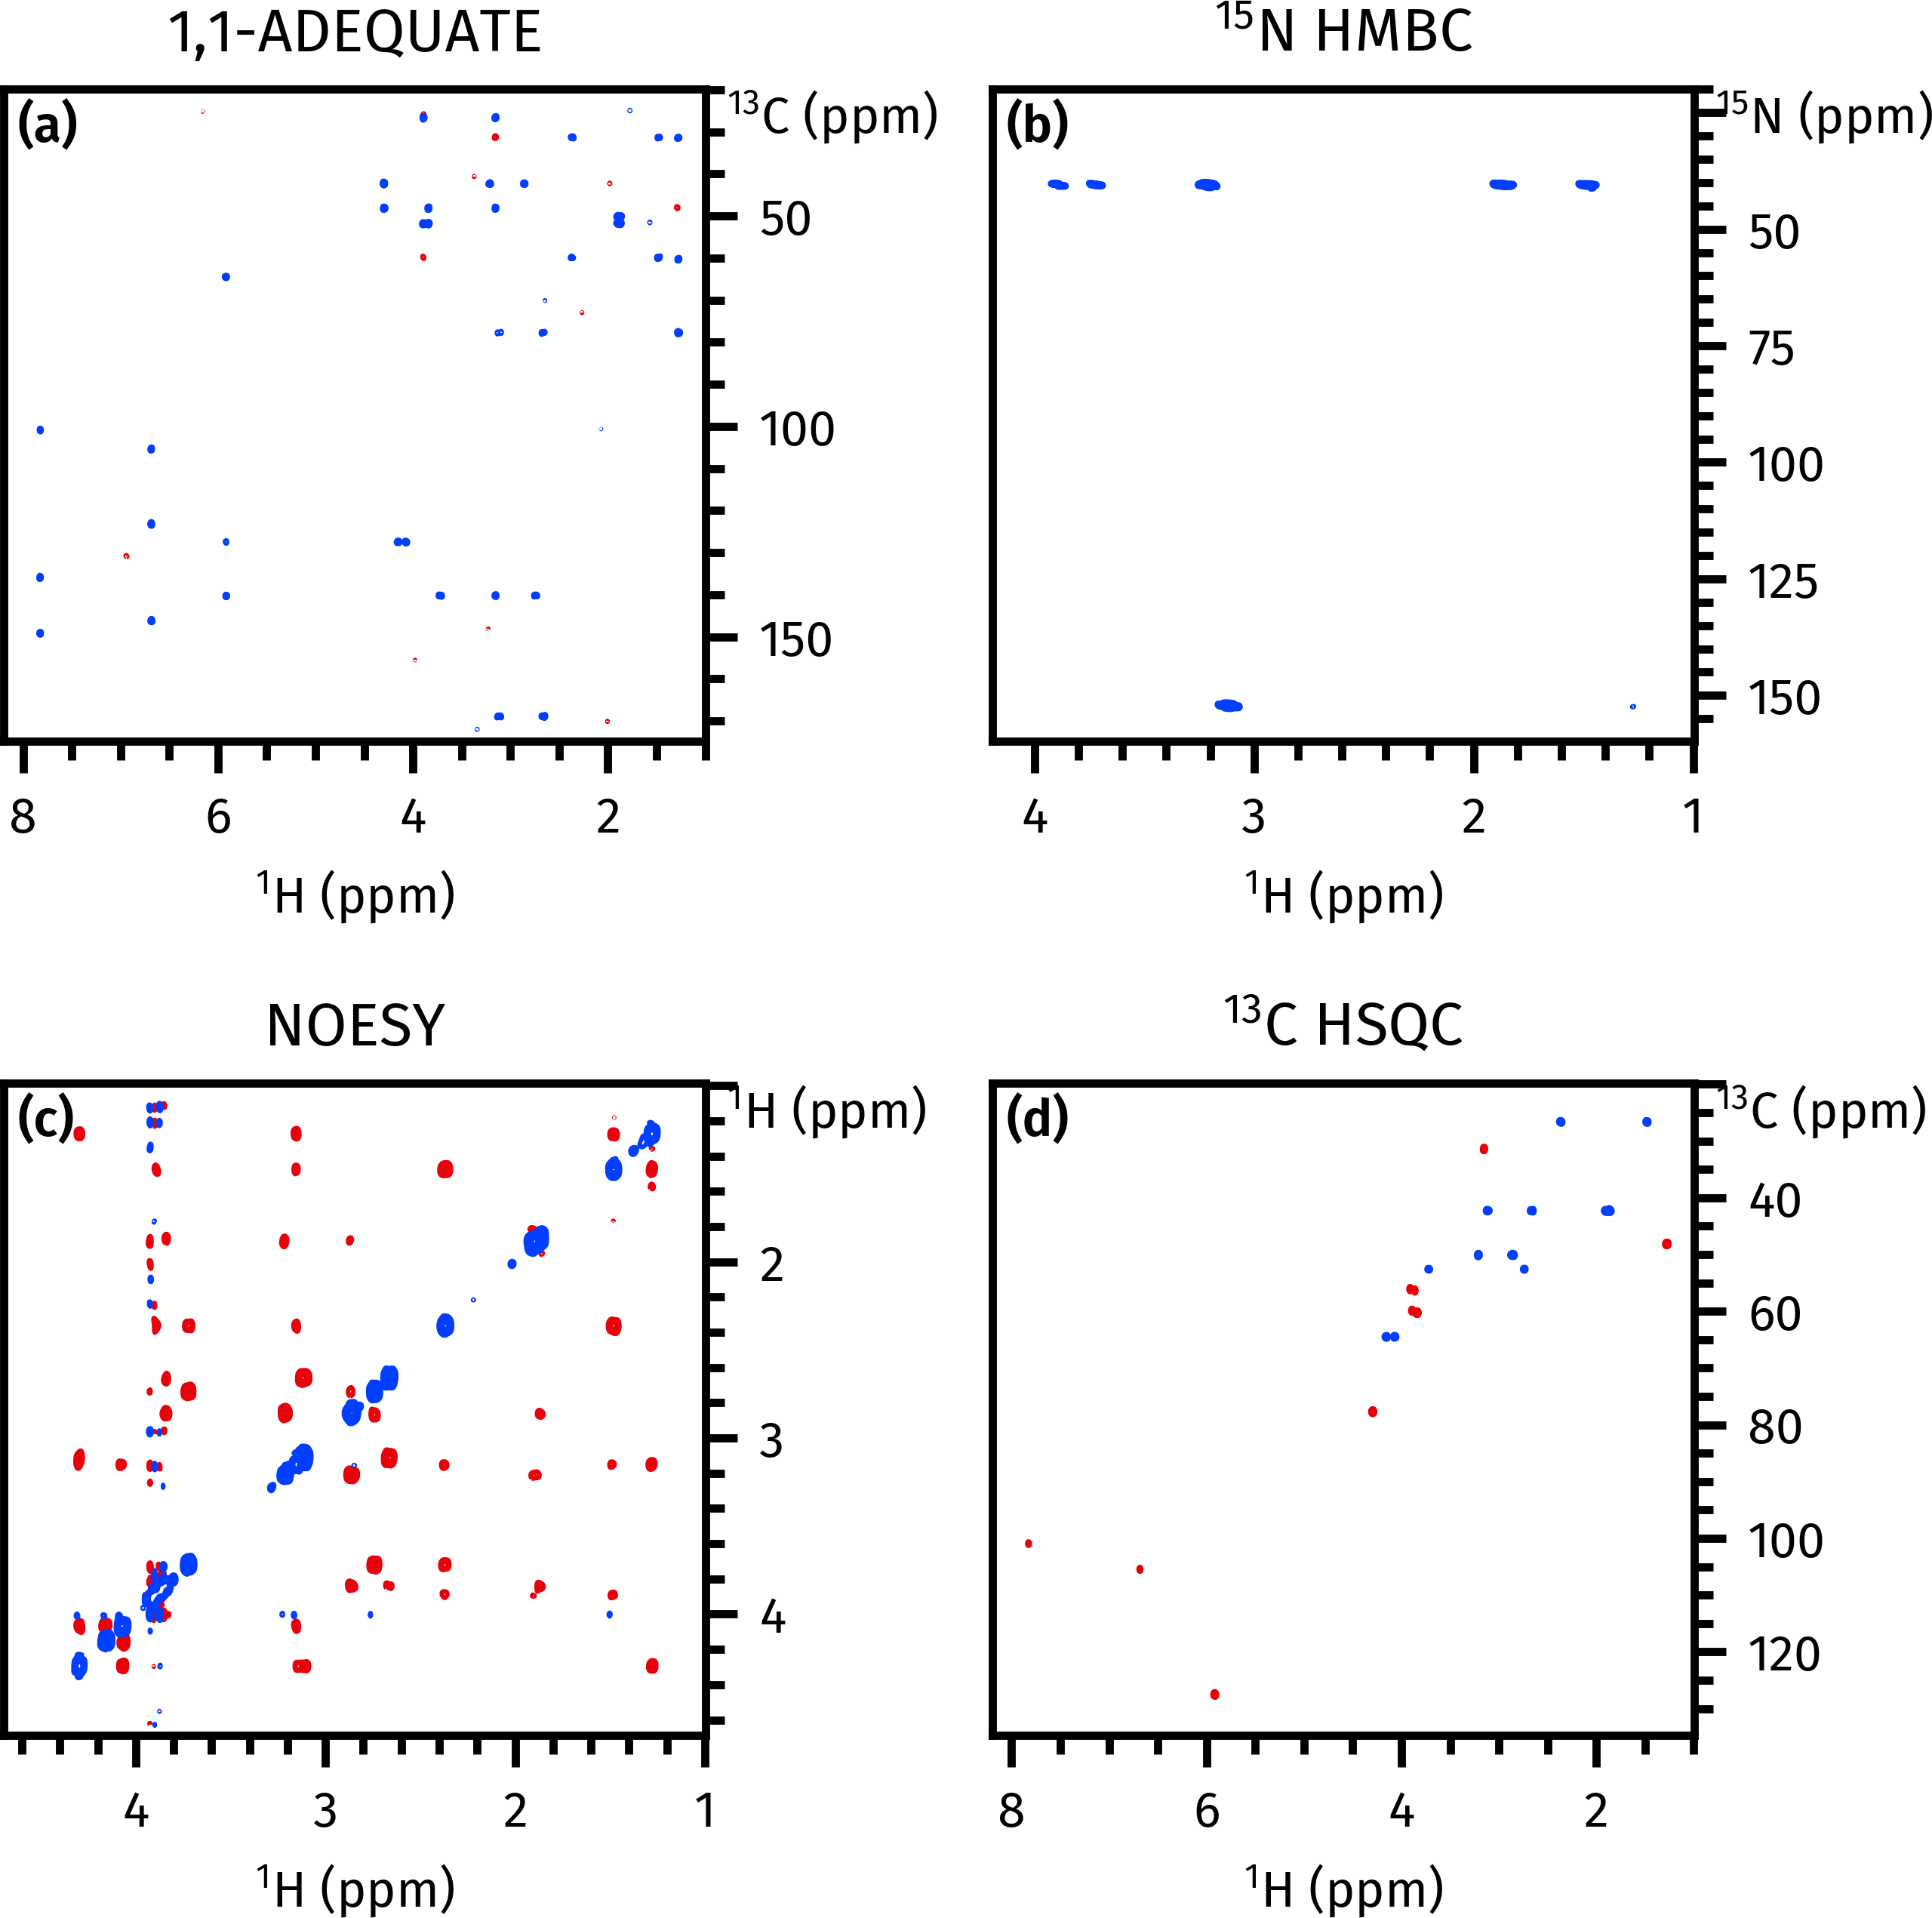
\includegraphics[width=0.7\textwidth]{abns.png}
    {\phantomsubcaption\label{fig:abns_adeq}}
    {\phantomsubcaption\label{fig:abns_n_hmbc}}
    {\phantomsubcaption\label{fig:abns_c_hmbc}}
    {\phantomsubcaption\label{fig:abns_c_hsqc}}
    \caption{
        Spectra obtained from the NOAH-4 \noahfour{A}{Bn}{N}{S} supersequence.
        \textbf{(\subref{fig:abns_adeq})} 1,1-ADEQUATE (16 transients).
        \textbf{(\subref{fig:abns_n_hmbc})} \nitrogen{} HMBC (12 transients).
        \textbf{(\subref{fig:abns_c_hmbc})} NOESY (2 transients, \SI{800}{\ms} mixing time).
        \textbf{(\subref{fig:abns_c_hsqc})} \carbon{} HSQC (2 transients).
        \brucine{}
    }
    \label{fig:abns}
\end{figure}


\section{ABBS comparison with and without DIPSI}

\begin{figure}[ht]
    \centering
    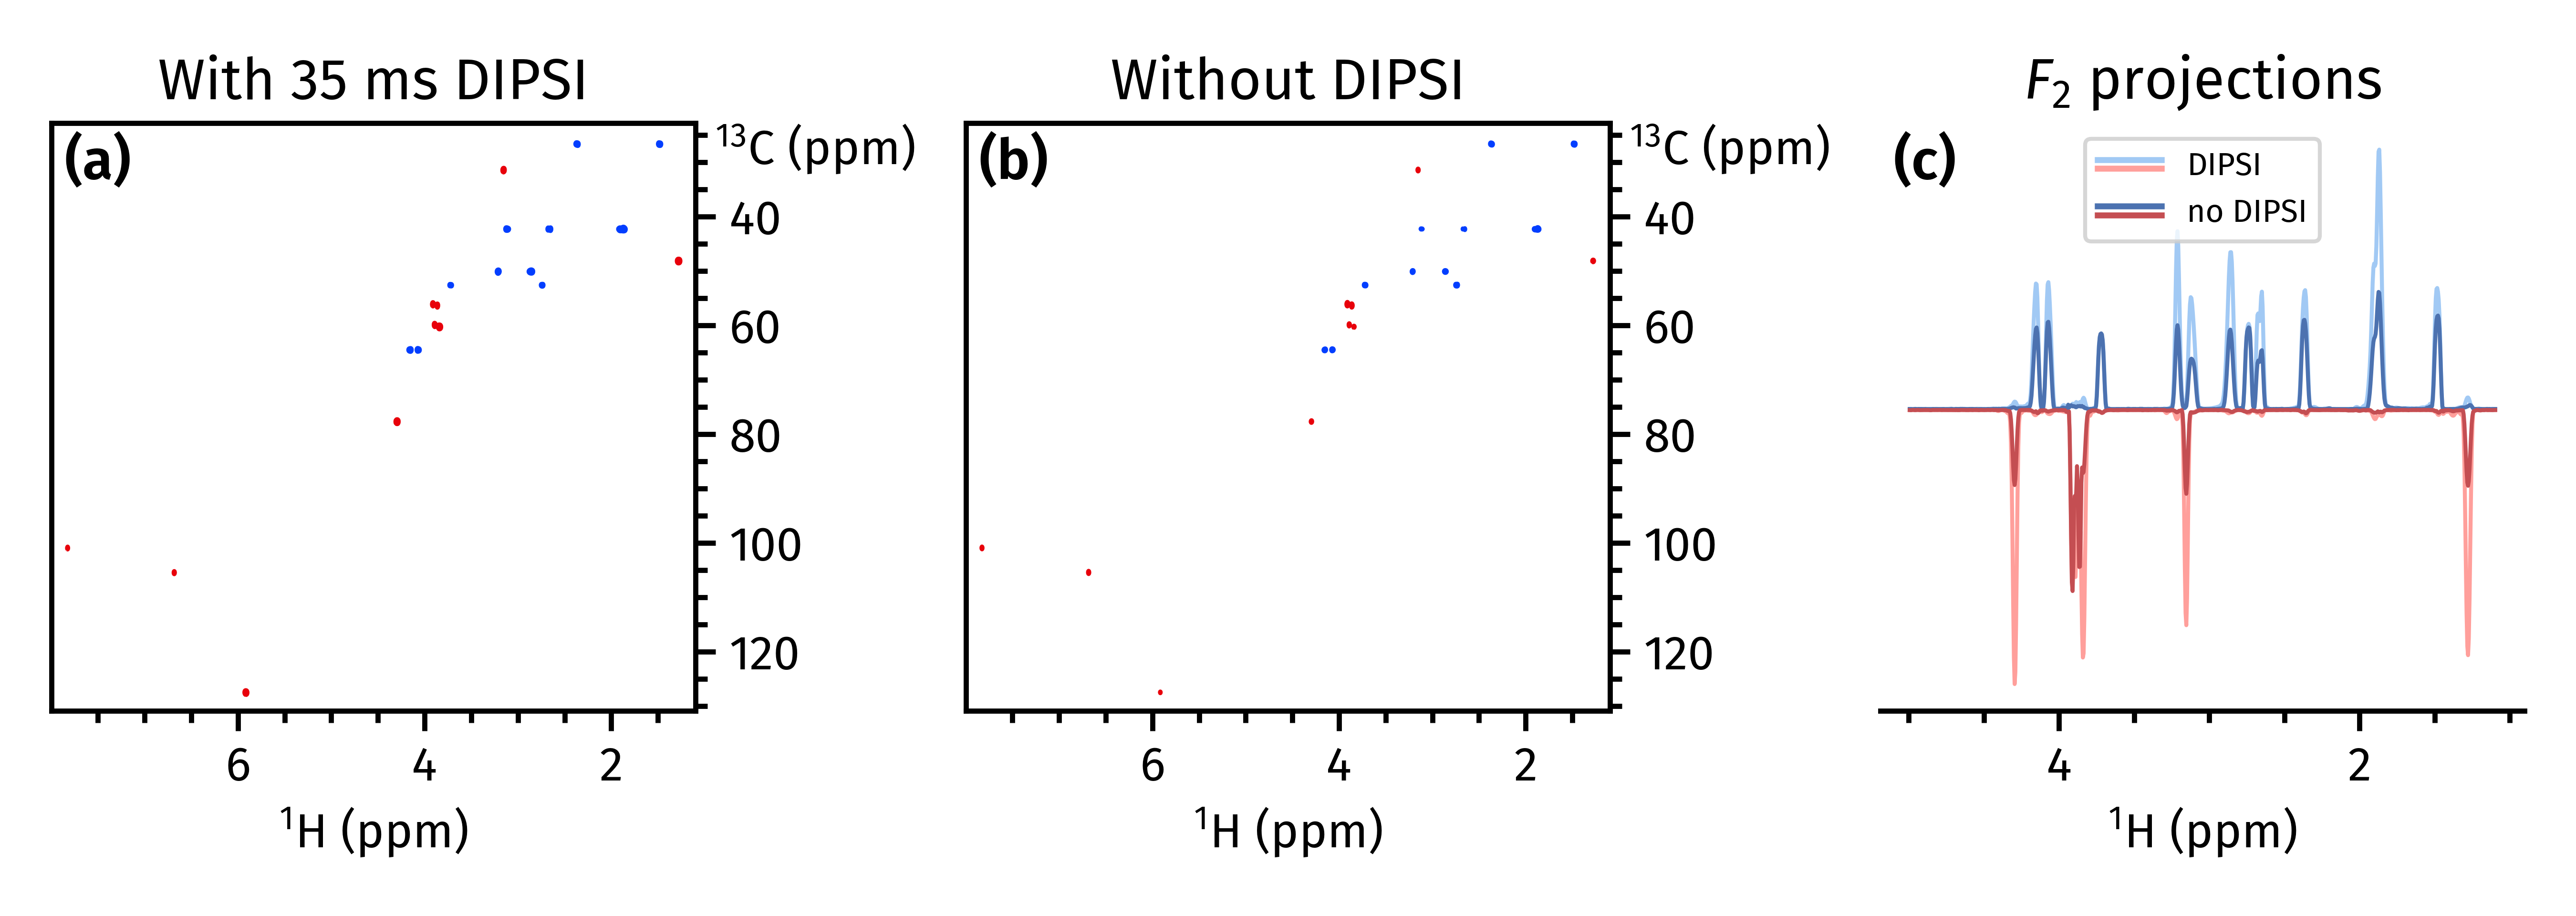
\includegraphics[width=\textwidth]{dipsi.png}
    {\phantomsubcaption\label{fig:dipsi_hsqc_nodipsi}}
    {\phantomsubcaption\label{fig:dipsi_hsqc_dipsi}}
    {\phantomsubcaption\label{fig:dipsi_projections}}
    \caption{
        \carbon{} HSQC spectra obtained from the NOAH-4 \noahfour{A}{Bn}{B}{S} experiment (\cref{fig:sequences_abbs}).
        \textbf{(\subref{fig:dipsi_hsqc_nodipsi})} Without DIPSI mixing between the ADEQUATE and \carbon{} HSQC modules.
        \textbf{(\subref{fig:dipsi_hsqc_dipsi})} With \SI{35}{\ms} DIPSI mixing between the ADEQUATE and \carbon{} HSQC modules (this spectrum is the same as in \cref{fig:abbs_c_hsqc}).
        \textbf{(\subref{fig:dipsi_projections})} Projections of the spectra in (\subref{fig:dipsi_hsqc_nodipsi}) and (\subref{fig:dipsi_hsqc_dipsi}) onto the $f_2$ axis.
        \brucine{}
    }
    \label{fig:dipsi}
\end{figure}

The average signal enhancement across all peaks is 88\% (\cref{fig:dipsi}).

Similar to results seen previously\autocite{Yong2021JMR}


% Fakesection SI bibliography
\AtNextBibliography{\small}
\printbibliography{}
\clearpage    % For some reason this is needed to make the last page number 'S5', not '5'

\end{refsection}

\end{document}
